\documentclass[10pt,twoside,a4paper,fleqn]{report}

\usepackage{braket}
\usepackage{graphicx}
\usepackage{parskip}
\usepackage{amssymb}
\usepackage{mathbbol}
\usepackage{xcolor}
\definecolor{darkyellow}{HTML}{FFB600}
\definecolor{emerald}{HTML}{32936F}
\usepackage{enumerate}
\usepackage{ragged2e}
\usepackage{eurosym}
\usepackage{amsmath}
\usepackage{amsmath,array}
\usepackage{apacite}
\usepackage{array}
\usepackage{caption}
\usepackage{fancyvrb}
\usepackage{float}
\usepackage{pgfplots} %for plotting
\pgfplotsset{compat=1.3}
\usepackage{xcolor,colortbl}
\definecolor{red1}{HTML}{FF0000}
\definecolor{red2}{HTML}{B20000}
\definecolor{red3}{HTML}{7F0000}
\definecolor{red4}{HTML}{FF3217}
\definecolor{red5}{HTML}{FF0D48}
\definecolor{blue1}{HTML}{0000FF}
\definecolor{blue2}{HTML}{0000B5}
\definecolor{blue3}{HTML}{000080}
\definecolor{blue4}{HTML}{3C00FF}
\definecolor{blue5}{HTML}{3C5DFF}
\definecolor{inputblue1}{HTML}{0000CC}
\definecolor{inputmixblue2}{HTML}{002DF7}
\definecolor{inputmixblue3}{HTML}{3C8BFF}
\definecolor{inputmixblue4}{HTML}{6730A8}
\definecolor{inputred1}{HTML}{970000}
\definecolor{inputmixred2}{HTML}{DF3100}
\definecolor{inputmixred3}{HTML}{C43335}
\definecolor{inputmixred4}{HTML}{DE366C}

\definecolor{examplered}{HTML}{FF3122}

\usepackage{siunitx} %for SI units
\usepackage{tcolorbox}
\newtcolorbox{redbox}{colback=red!5!white,colframe=red!75!black}
\newtcolorbox{bluebox}{colback=blue!5!white,colframe=blue!75!black}
\newtcolorbox{greenbox}{colback=green!5!white,colframe=green!75!black}

\usepackage{filecontents} %for data loading
\begin{filecontents}{datax.dat}
0.06941, 28, 0.44096, 30, 0.15165, 25
0.04389, 146, 0.32707, 132,0.10722, 109
0.02823, 3622, 0.08416, 3478, 0.02086, 2997
0.01008, 17838, 0.005179, 17566, 0.01494, 14721
0.00165, 89130,0.0015799, 88216, 0.003327, 74009
0.00156, 444646, 0.0015601, 439060, 0.001578, 370813
%previous 3rd row: 0.04951, 728, 0.224107, 642, 0.020864, 601
\end{filecontents}

%This table contains amplitude data for delta=0.1 until delta=0.4
\begin{filecontents}{gaussamp1.dat}
-4,0.8101, 0.63905, 0.48944, 0.36085
-3, 0.27205, 0.3192, 0.32442, 0.29198
-2, 0.08826, 0.16093, 0.20988, 0.24121
-1, 0.03209, 0.07956, 0.1374, 0.1944
0, 0.00894, 0.03873, 0.09311, 0.16254
1, 0.02983, 0.0821, 0.13932, 0.19491
2, 0.08916, 0.16236, 0.20698, 0.24247
3, 0.27048, 0.31959, 0.31812, 0.29601
4, 0.8101, 0.63905, 0.48944, 0.36085 
\end{filecontents}

%This table contains probability data for delta=0.5 until delta=0.9
\begin{filecontents}{gaussprobs.dat}
-4, 0.000100, 0.001600, 0.007920, 0.025390, 0.063610 
-3, 0.000880, 0.006500, 0.018960, 0.038630, 0.063770 
-2, 0.008090, 0.025810, 0.043210, 0.058350, 0.062440
-1, 0.073020, 0.103850, 0.101660, 0.085750, 0.061800 
0, 0.653810, 0.407530, 0.239850, 0.129960,  0.063010 
1, 0.072500, 0.101520, 0.104090, 0.087560, 0.062780
2, 0.007950, 0.025120, 0.044750, 0.056280, 0.062690
3, 0.000870, 0.006420, 0.018530, 0.038770, 0.061890
4, 0.000100, 0.001600, 0.007920, 0.025390, 0.063610
\end{filecontents}

                     
%This table contains amplitude data for delta=0.5 until delta=0.9
\begin{filecontents}{gaussamp2.dat}
-4, 0.2492,0.15792, 0.09039,0.03688,0.00949, 0.0
-3, 0.24862, 0.19771, 0.13755,0.08068,0.02966, 0.0
-2, 0.2514, 0.23879,  0.21133,0.16223,0.09132, 0.0
-1, 0.25012, 0.29307,0.32105,0.31975,0.27052, 0.0
0,  0.2504,0.3577,0.48748,0.64152,0.80941, 1.0
1, 0.24815,0.29384,0.32165,0.32011,0.27019, 0.0
2, 0.24833,0.24276,0.20698, 0.16016,0.08803, 0.0
3, 0.25112, 0.1968,0.13733, 0.07576,0.03225, 0.0
4, 0.2492,0.15792,0.09039, 0.03688,0.00949, 0.0
\end{filecontents}

\begin{filecontents}{gauss2.dat}
0.0043579, -3
0.022322, -2
0.11434, -1
0.58566, 0
0.11434, 1
0.11434, 1
0.022322, 2
0.022322, 2
0.0043579, 3
\end{filecontents}


% Defining some new mathematics commands
\newcommand*{\colvec}[1]{\begin{pmatrix}#1\end{pmatrix}}
\newcommand*{\0}{$\ket{0}$}
\newcommand*{\1}{$\ket{1}$}
\newcommand*{\Title}{A very long table heading}%
\newcommand*{\TitleInParbox}{\parbox[c]{0.3\linewidth}{\Title}}%
\usepackage{array}
\newcolumntype{L}[1]{>{\raggedright\let\newline\\\arraybackslash\hspace{0pt}}m{#1}}
\newcolumntype{C}[1]{>{\centering\let\newline\\\arraybackslash\hspace{0pt}}m{#1}}
\newcolumntype{R}[1]{>{\raggedleft\let\newline\\\arraybackslash\hspace{0pt}}m{#1}}


\usepackage[english,bt]{ethidsc} % Special IDSC styles and commands      
								 % {german}/english: language of headings, etc.
								 % {st}/bt/mt: {semester}/bachelor/master thesis
							
% Page header (don't change)____________________________________________________
\setlength{\parindent}{0em}                 % Disable parindent
\rhead[\nouppercase{\rightmark}]{\thepage}  % Special headings
\lhead[\thepage]{\nouppercase{\leftmark}}   % Special headings
\cfoot{}                                    % Special headings


% Title page (please fill in)___________________________________________________
\title{DRAFT:\\Quantum-enhanced machine learning:
Implementing a quantum k-nearest neighbour algorithm}


\studentA{Mark Fingerhuth}
\ethidA{I6082973}
\semesterA{5}
\emailA{m.fingerhuth@student.maastrichtuniversity.nl}

\supervision{Prof. Francesco Petruccione\\ Dr. Fabrice Birembaut}
\date{January 2017}

%\identification{} 		% Project identifier

%\infopage %includes the last page
%\declaration

% Begin  document________________________________________________________________
\begin{document}

\maketitle 							% Create title page


% Preamble______________________________________________________________________

\pagenumbering{roman} 				% Begin roman page numbering (i,ii,...)

%---------------------------------------------------------------------------
% Preface

\chapter*{Preface}

Blah blah \dots

 \cleardoublepage

%---------------------------------------------------------------------------
% Table of contents

 \setcounter{tocdepth}{2}
 \tableofcontents

 \cleardoublepage

%---------------------------------------------------------------------------
% Abstract

\chapter*{Abstract}
 \addcontentsline{toc}{chapter}{Abstract}

NEEDS MODIFICATION!

Quantum machine learning, the intersection of quantum computation and classical machine learning,
bears the potential to provide more efficient ways to deal with big data through the use of quantum
superpositions, entanglement and the resulting quantum parallelism. The proposed research will
attempt to implement and simulate two quantum machine learning routines and use them to solve
small machine learning problems. That will establish one of the earliest proof-of-concept studies in
the field and demonstrate that quantum machine learning is already implementable on small-scale
quantum computers. This is vital to show that an extrapolation to larger quantum computing devices
will indeed lead to vast speed-ups of current machine learning algorithms.

 \cleardoublepage

%---------------------------------------------------------------------------
% Symbols

\chapter*{Nomenclature}\label{chap:symbole}
 \addcontentsline{toc}{chapter}{Nomenclature}

\section*{Symbols}
\begin{tabbing}
 \hspace*{1.6cm} \= \hspace*{8cm} \= \kill
 $\otimes$ \> Tensor product \\[0.5ex]
 $i$ \> Imaginary unit \> $i=\sqrt{-1}$ \\[0.5ex]
 $\dagger$ \> Hermitian conjugate \> Complex conjugate transpose \\[0.5ex]
 $!$ \> Factorial \> e.g. 3! = 3*2*1 \\[0.5ex]
\end{tabbing}

\section*{Indicies}
\begin{tabbing}
 \hspace*{1.6cm}  \= \kill
 a \> Ambient \\[0.5ex]
 air \> Air
\end{tabbing}

\section*{Acronyms and Abbreviations}
\begin{tabbing}
 \hspace*{1.6cm}  \= \kill
 QML \> Quantum machine learning \\[0.5ex]
 QC \> Quantum computer \\[0.5ex]
 Prob \> Probability \\[0.5ex]
 PM \> Post-measurement \\[0.5ex]
 HD \> Hamming distance \\[0.5ex]
 CM \> Conditional measurement \\[0.5ex]
 CNOT \> Controlled NOT gate \\[0.5ex]
 CCNOT \> Controlled controlled NOT gate (Toffoli gate) \\[0.5ex]
 CU \> Controlled U gate (where U can be any unitary quantum gate) \\[0.5ex]
\end{tabbing}

 \cleardoublepage

%---------------------------------------------------------------------------


% Chapters______________________________________________________________________

\pagestyle{fancy}               	% Fancy headings
\pagenumbering{arabic}				% Begin arabic page numbering (1,2,...)

\chapter{Introduction}\label{sec:introduction}

The ability to recognise familiar faces, to understand spoken language and to distinguish types of vegetables comes naturally to humans, although these processes of pattern recognition and classification are inherently complex. Machine learning (ML), a subdiscipline of artificial intelligence, is concerned with the development of algorithms that perform these types of tasks, thus enabling computers to find and recognise patterns in data and classify unknown inputs based on previous training data. Such algorithms make the core of e.g. human speech recognition and recommendation engines as used by Amazon \cite{graves2013speech,linden2003amazon}.
% and algorithms that can predict heart disease from real-time electrocardiograms \citep{acharya2015integrated, pazzani2007content}.

According to \citeA{bigdata}, approximately 2.5 quintillions (${10}^{18}$) bytes of digital data are created every day. This growing number implies that many areas dealing with data will eventually require advanced algorithms that can make sense of data content, retrieve patterns and reveal correlations. However, most ML algorithms involve the execution of computationally expensive operations and doing so on large data sets inevitably takes a lot of time \cite{bekkerman2011scaling}. Thus, it becomes increasingly important to find efficient ways of dealing with big data.
%and/or reduce the computational complexity of the algorithms.

A promising solution is the use of quantum computation which has been researched intensively in the last few decades. Quantum computers (QCs) use quantum mechanical systems and their unique properties to manipulate and process information in ways that are impossible for classical computers. Analogous to a classical computer manipulating bits, a quantum computer makes use of so-called quantum bits (qubits). Bits and qubits are both binary entities meaning they can only take the values 0 and 1. However, a non-probabilistic classical bit can only take one of these values at a time whereas a qubit can also be found in a linear superposition of the two states.

%\begin{equation}
%\label{equ: simplequbit}
%\ket{q} = \alpha \ket{0} + \beta \ket{1}
%\end{equation}
%where $\alpha$ and $\beta$ are complex numbers and often referred to as amplitudes. When measuring qubit $\ket{q}$ it will take the value \0 with a probability of ${|\alpha|}^{2}$ and \1 with a probability of ${|\beta|}^{2}$. Since the total probability has to sum to unity, the normalization condition ${|\alpha|}^{2} + {|\beta|}^{2} =  1$ must be satisfied at all times.

This property gives rise to quantum parallelism, which enables the execution of certain operations on many quantum states at the same time. Despite this advantage, the difficulty in quantum computation lies in the retrieval of the computed solution since a measurement of a qubit collapses it into a single classical bit and thereby destroys information about its previous superposition. Several quantum algorithms have been proposed that provide exponential speed-ups when compared to their classical counterparts with Shor's prime factorization algorithm being the most famous \cite{shor1994}.
%As another example, Grover's quantum database search algorithm enables finding a single element in a list of $N$ elements within roughly $\sqrt{N}$ quantum mechanical steps instead of $N$ classical steps \citep{grover}.
Thus, quantum computation has the potential to improve computational power, speed up the processing of big data and possibly solve certain problems that are practically unsolvable on classical computers e.g. computationally-exhaustive optimisation problems such as the well-known travelling salesman problem with more than 1000 cities \cite{kieu2006quantum}.

%for the QML toolbox to be complete a quantum algorithm to solve systems of linear equations is needed since most ML algorithms rely on solving those.

Considering these advantages, the combination of quantum computation and classical ML into the new field of quantum machine learning (QML) seems almost natural. More specifically, one speaks of quantum-enhanced machine learning when quantum computation is used to improve classical ML algorithms. Yet, both fields are mutually beneficial to each other since classical ML can also be used to improve aspects of quantum computation. For example, \citeA{las2016genetic} showed that a classical genetic algorithm can be used to reduce the experimental error in quantum logic gates. However, this thesis will only focus on the field of quantum-enhanced machine learning.

%There are currently two main ideas on how to merge quantum computation with ML, namely a) running the classical algorithm on a classical computer and outsourcing only the computationally intensive task to a QC or b) executing the quantum version of the entire algorithm on a QC. Current QML research mostly focusses on the latter approach by developing quantum algorithms that tap into the full potential of quantum parallelism.

\section{Motivation}
\label{sec:motivation}

Classical ML is a very practical topic since it can be directly tested, verified and implemented on any commercial classical computer. So far, QML has been of almost entirely theoretical nature since the required computational resources are not yet in place. To yield reliable solutions QML algorithms often require a huge number of error-correcting qubits and some quantum data storage such as the proposed quantum random access memory (qRAM) \cite{qRAM}. However, to date the maximum number of e.g. superconducting qubits reportedly used for calculation is nine, the D-Wave II quantum annealing device delivers 1152 qubits but can only solve a narrow class of problems, and a qRAM has not been developed yet \cite{hydrogensimulation, dwave2}. Furthermore, qubit error-correction is still a very active research field, and most of the described preliminary QCs deal with non-error-corrected qubits with short lifetimes and are, thus, impractical for large QML implementations.

Until now there have been only a few experimental verifications of QML algorithms that establish proof-of-principle. \citeA{Li2015} successfully distinguished handwritten digits using a quantum support vector machine on a four-qubit nuclear magnetic resonance test bench. In addition, \citeA{Cai2015} were first to experimentally demonstrate quantum machine learning on a photonic QC and showed that the distance between two vectors and their inner product can indeed be computed quantum mechanically. Lastly, \citeA{Riste2015} solved a learning parity problem with five superconducting qubits and found that a quantum advantage can already be observed in non-error-corrected systems.

%Consequently,
Considering the gap between the number of proposed QML algorithms and the few experimental realisations, it becomes important to find QML problems which can already be implemented on small-scale QCs. Hence, the purpose of this research is to provide proof-of-principle implementations and simulations of selected QML algorithms on small datasets. For this purpose, the $k$-nearest neighbour algorithm, one of the simplest ML algorithms, was chosen as a good minimal example for implementation and quantum simulation. This is a necessary step in the attempt to shift QML from a purely theoretical research area to a more applied field such as classical ML.

\section{Research question}
\label{sec:researchquestion}


%Don't know where this should go!

%Matthias Troyer citation for this part:

%Finding optimal ways of compiling a given quantum algorithm as well as designing a high-level programming language or environment similar to that of classical computer code editors is called \emph{quantum software engineering}.

In light of the theoretical nature of current QML research and the small number of experimental realisations, this research will address the following question:

%NARROW DOWN THE RESEARCH QUESTION!
\centering\textbf{How can a k-nearest neighbour quantum machine learning algorithm be implemented on small-scale quantum computers?}

%Alternatives:
%Is it possible to experimentally demonstrate that two QML algorithms proposed by \cite{Schuld2014, Schuld2016} can already solve a small ML problem using classical simulation or IBMs quantum processor?
%Is it possible to already implement and solve a small ML problem on IBMs publicly available quantum computer?

\justify
The following sections will introduce the necessary theoretical foundations, and the tools used to answer this research question. 

%\cleardoublepage
\chapter{Theoretical Foundations}\label{sec:theory}
\emph{Please note that all concepts introduced in Section~\ref{subsec:qubits} and Section~\ref{subsec:quantumlogicgates} can be found in any standard textbook on quantum information and will, therefore, not be referenced individually. Both of these sections are mainly based on the textbook by \citeA{nielsen2010quantum}.}
\section{Quantum bits}
\label{subsec:qubits}
\subsection{Single qubit systems}
\label{subsubsec:qubits}

Classical computers manipulate bits, whereas quantum computer's most fundamental unit is called a \emph{quantum bit}, often abbreviated as \emph{qubit}. Instead of 0 and 1, qubit states are denoted \0 and \1 for reasons that will be outlined later.
%A non-probabilistic classical bit is a binary entity and can take either the value 0 or 1. Qubits are also binary entities but they can also be in a superposition of the two states. In contrast to classical bits, the two fundamental qubit states are denoted \0 and \1 for reasons outlined later.

A good example of a physical implementation of a qubit is the single electron of a hydrogen atom sketched in Fig.~\ref{img:qubitatom}. Usually, the electron is found in its ground state which one can define as the \0 state of the qubit. By using a laser pulse, the electron can be excited into the next higher valence shell which one can define as the \1 state of the qubit. After some time $t$ the electron will decohere to its ground state \0 which is called the \emph{longitudinal coherence} or \emph{amplitude damping time} and is an important parameter for measuring qubit lifetimes \cite{chuanglecturenotes}.

\begin{figure}[!ht]
       \centering
       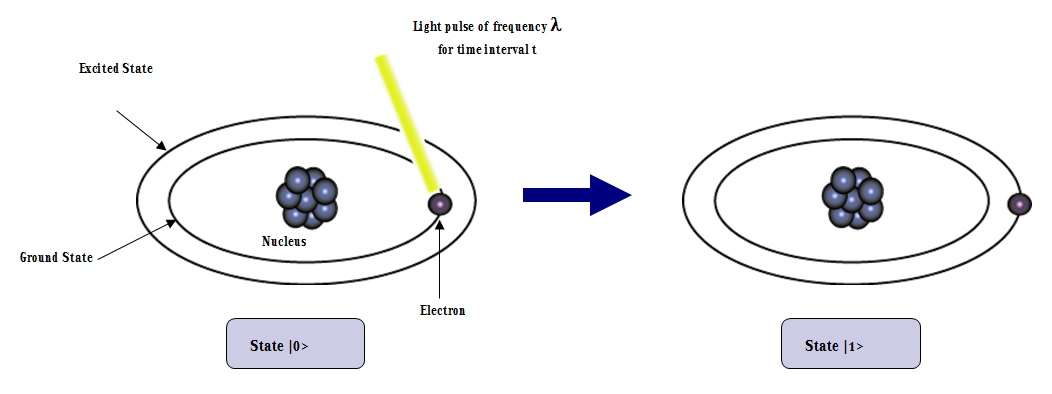
\includegraphics[scale=0.35]{img/qubitimplementation.jpeg}
       \caption[]{\label{img:qubitatom} A simple example of a physical qubit using the single valence electron of a hydrogen atom. Thereby, the electron's ground state can be defined as the \0 state of the qubit. By using a laser pulse, the electron can be excited into the next higher valence shell which can be defined as the qubit's \1 state. \textsuperscript{1}}
\end{figure}
\footnotetext[1]{Reprinted from RF Wireless World, n.d., Retrieved December 23, 2016, from \url{http://www.rfwireless-world.com/Terminology/Difference-between-Bit-and-Qubit.html}. Copyright 2012 by RF Wireless World.}

\pagebreak
A classical non-probabilistic bit can only take one of the two possible values at once. In contrast, qubits obey the laws of quantum mechanics, which gives rise to the important property that - besides being a definite \0 or \1 - they can also be in a superposition of the two states. Mathematically this is expressed as the linear combination of the states \0 and \1:
\begin{equation}
\label{equ: simplequbit}
\ket{\psi} = \alpha \ket{0} + \beta \ket{1}\, ,
\end{equation}
where $\alpha$ and $\beta$ are complex coefficients ($\alpha, \beta \in \mathbb{C}$) and are often referred to as amplitudes. Any amplitude $\eta$ can be further subdivided into a complex phase factor $e^{i\phi}$ and a non-negative real number $e$ such that
\begin{equation}
\label{equ: amplitude}
\eta = e^{i\phi}e\, .
\end{equation}
 
In Eq.~\ref{equ: simplequbit}, \0 is the Dirac notation for the qubit being in state 0 and can be represented as a two-dimensional vector in a complex two-dimensional vector space (called Hilbert space $\mathcal{H}_{2}$). First defined by \citeA{dirac1939new}, the object
\begin{equation}
\ket{\phi}\, ,
\end{equation}
is called a \emph{ket} and its Hermitian conjugate
\begin{equation}
\ket{\phi}^\dagger = \bra{\phi}\, ,
\end{equation}
is called a \emph{bra}. The Hermitian conjugate, denoted with a dagger ($\dagger$), of some e.g. two-dimensional column vector $c$ with complex entries $c_1$ and $c_2$:
\begin{equation}
c = \colvec{c_1\\c_2}\, ,
\end{equation}
is obtained by complex conjugating each entry and then transposing vector $c$:
\begin{equation}
c^\dagger = \colvec{c_1\\c_2}^\dagger = \begin{pmatrix}c_1^* & c_2^*\end{pmatrix}\, ,
\end{equation}
where complex conjugates are denoted with an asterisk ($*$). The Hermitian conjugate is defined for vectors as well as square matrices.

The inner product of a bra and a ket is called a \emph{bra-ket} and is written
\begin{equation}
\braket{\phi|\phi}
\end{equation}
Note that all later sections will make heavy use of this \emph{bra-ket notation}.

The quantum states \0 and \1 are called the computational basis states and they constitute an orthonormal basis of $\mathcal{H}_{2}$. When a qubit is expressed in terms of the two states \0 and \1 it is said to be in its \emph{standard basis}. For the sake of clarity, \0 and \1 can be represented as the 2-D vectors
\begin{equation}
\label{equ: 0and1kets}
\ket{0} \doteq  \colvec{1\\0} \quad \mathrm{and} \quad \ket{1} \doteq \colvec{0\\1} \, .
\end{equation}

Note that a ket and its vector representation are not the same object since a well-defined vector requires a basis whereas a ket does not demand specification of a basis. This thesis will make use of the $\doteq$ symbol when switching between the two different ways of representing a ket. Substituting the vectors from Eq.~\ref{equ: 0and1kets} into Eq.~\ref{equ: simplequbit} yields the vector representation of $\ket{\psi}$:
\begin{equation}
\label{equ: simplequbitvector}
\ket{\psi} \doteq \alpha \colvec{1\\0} + \beta \colvec{0\\1} = \colvec{\alpha\\\beta}\, .
\end{equation}

In the cases $\alpha = 1$ or $\beta = 1$ the qubit is not in a superposition but in the definite state \0 or \1 respectively. However, if for example $\alpha = \frac{1}{\sqrt{2}}$ and $\beta = \frac{i}{\sqrt{2}}$ the qubit is in a quantum superposition, impossible to achieve with a classical computer. This leads to another important qubit lifetime parameter - the \emph{transversal coherence} or \emph{phase damping time}. It is measured by preparing the equal superposition $\frac{\ket{0}+\ket{1}}{\sqrt{2}}$ and due to unavoidable interaction with the environment after some time $t$ the quantum behaviour will be lost, and the state will either be a definite \0 or \1 \cite{chuanglecturenotes}. The process of losing quantum behaviour is called \emph{decoherence}.

However, even though a qubit can be in a superposition of \0 and \1, when measured it will take the value \0 with a probability of
\begin{equation}
\label{equ:bornrule0}
\mathrm{Prob}(\ket{0}) = {|\alpha|}^{2}\, ,
\end{equation}
and \1 with a probability of 
\begin{equation}
\label{equ:bornrule1}
\mathrm{Prob}(\ket{1}) = {|\beta|}^{2}\, .
\end{equation}

The fact that the probability of measuring a particular state is equal the absolute value squared of the respective amplitude was first postulated by \cite{born1954statistical} and, thus, is called Born rule. Since the total probability of measuring any value has to be 1, the normalisation condition
\begin{equation}
\label{equ: normalization}
{|\alpha|}^{2} + {|\beta|}^{2} =  1\, ,
\end{equation}
must be satisfied. Therefore, a qubit is inherently probabilistic but when measured it collapses into a single classical bit (0 or 1). It follows that a measurement destroys information about the superposition of the qubit (the values of $\alpha$ and $\beta$). This constitutes one of the main difficulties when designing quantum algorithms since only limited information can be obtained about the final states of the qubits in the quantum computer.

Using spherical polar coordinates, a single qubit can be visualized on the so-called Bloch sphere by parameterising $\alpha$ and $\beta$ in Eq.~\ref{equ: simplequbit} as follows:
\begin{equation}
\label{equ: blochqubit}
\ket{\psi} = \cos\frac{\theta}{2} \ket{0} + e^{i \phi} \sin\frac{\theta}{2} \ket{1}\, .
\end{equation}
The Bloch sphere has a radius of 1 and is, therefore, a unit sphere. The \0 qubit state is defined to lie along the positive $\hat{z}$-axis and the \1 state is defined to lie along the negative $\hat{z}$-axis as labelled in Fig.~\ref{fig:blochsphere}. At this point, it is important to note that these two states are mutually orthogonal in $\mathcal{H}_{2}$ even though they are not orthogonal on the Bloch sphere. 

Qubit states on the Bloch equator such as the $\hat{x}$ and $\hat{y}$ coordinate axes represent equal superpositions where \0 and \1 both have measurement probabilities equal to $0.5$. The $\hat{x}$-axis for example represents the equal superposition $\ket{q} = \frac{1}{\sqrt{2}} \ket{0} + \frac{1}{\sqrt{2}} \ket{1}$. As illustrated in Fig.~\ref{fig:blochsphere} any arbitrary 2-D qubit state $\ket{\psi}$ can be decomposed into the polar angles $\theta$ and $\phi$ and visualized as a vector on the Bloch sphere. Such an object is called the Bloch vector of the qubit state $\ket{\psi}$. The Bloch sphere will be the main visualization tool for qubit manipulations in this thesis.

\begin{figure}[!ht]
       \centering
       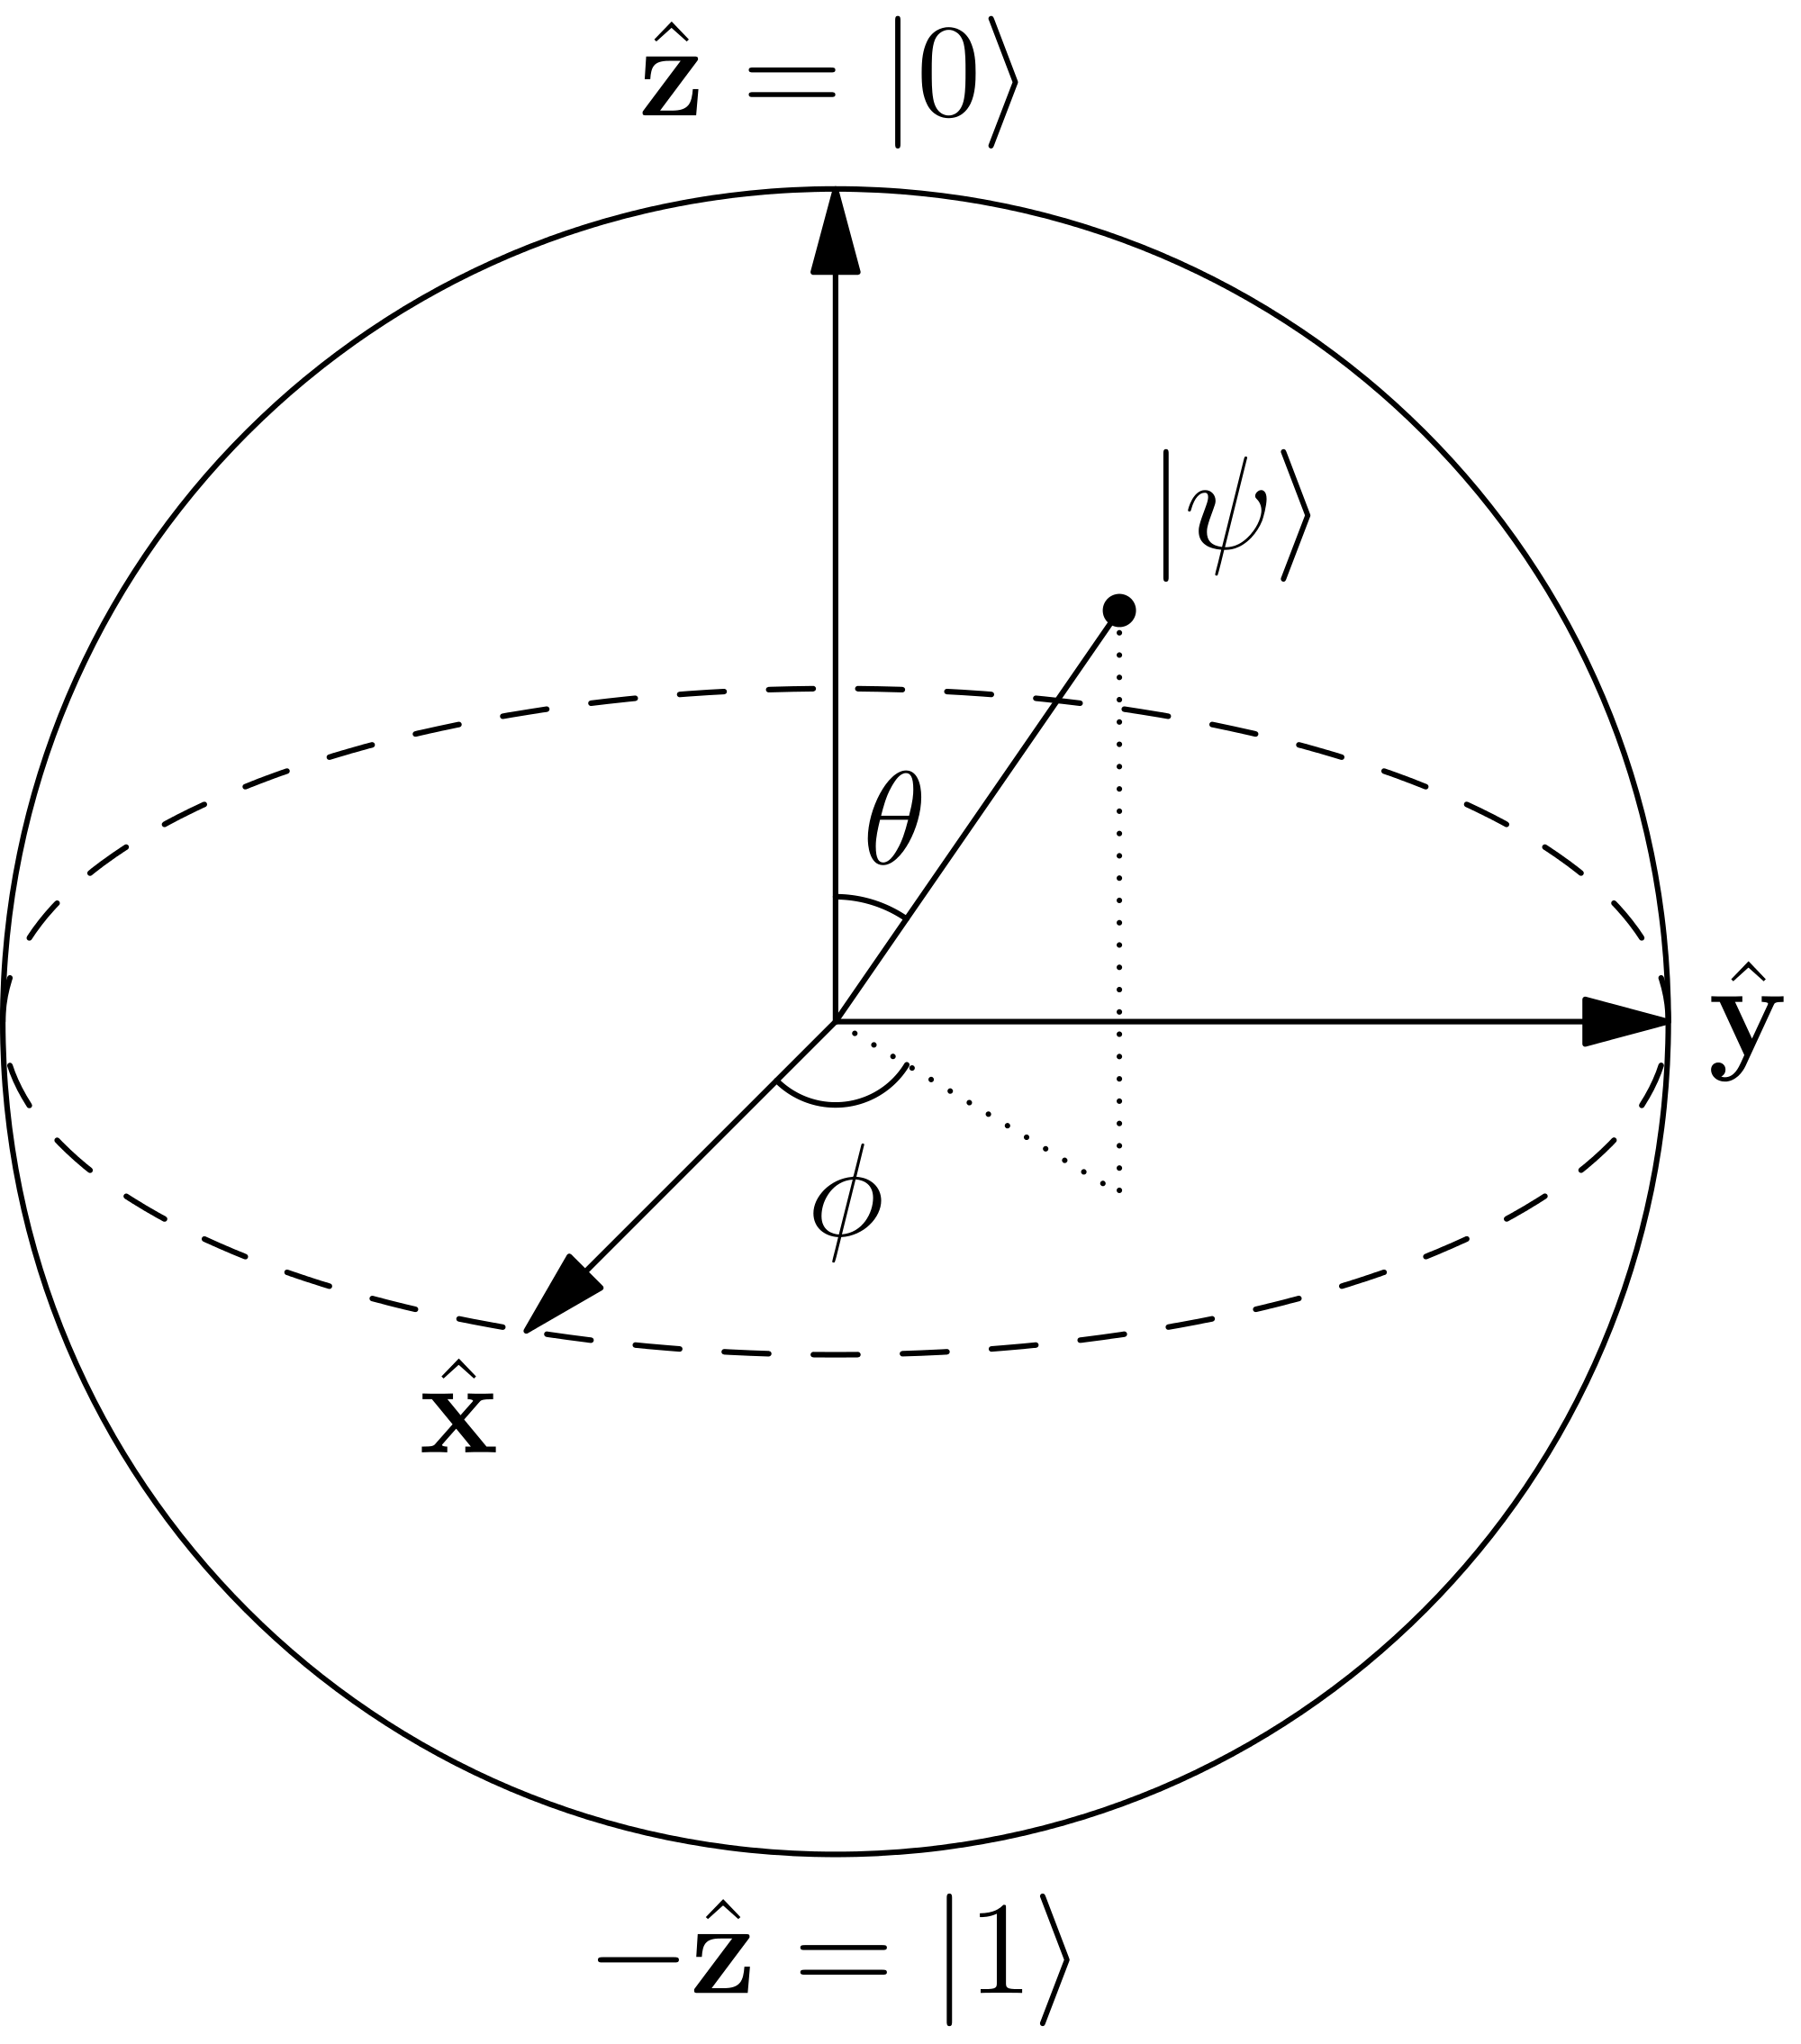
\includegraphics[scale=0.11]{img/blochsphere.png}
       \caption[]{\label{fig:blochsphere} An arbitrary single-qubit state $\ket{\psi} = \alpha \ket{0} + \beta \ket{1}$ can be visualized on the Bloch sphere by parameterising $\alpha = \cos\frac{\theta}{2}$ and $\beta = e^{i \phi} \sin\frac{\theta}{2}$ where $\theta$ is the polar and $\phi$ the azimuthal angle in spherical polar coordinates.\footnotemark[2]}
\end{figure}
\footnotetext[2]{Reprinted from Wikipedia, n.d., Retrieved September 7, 2016, from \url{https://en.wikipedia.org/wiki/Bloch_Sphere}. Copyright 2012 by Glosser.ca.}
\newpage

Similar to logic gates in a classical computer, a QC manipulates qubits, by means of quantum logic gates which will be introduced in detail in Section~\ref{subsec:quantumlogicgates}. Generally, an arbitrary quantum logic gate $U$ acting on a single qubit state is a unitary transformation which can be represented as a $2\times2$ matrix:
\begin{equation}
\label{equ:generalquantumgate}
U \doteq \begin{pmatrix}
 a & b \\ 
 c & d
 \end{pmatrix}\, ,
\end{equation}
whose action on $\ket{\psi}$ is defined as:
\begin{equation}
\label{equ:unitarytransformation}
U \ket{\psi} \doteq \begin{pmatrix}
 a & b \\ 
 c & d
 \end{pmatrix} \colvec{\alpha\\\beta} = \colvec{a\alpha+b\beta\\c\alpha+d\beta}\, .
\end{equation}

The matrix $U$ must be unitary which means that its determinant must equal unity:
\begin{equation}
\label{equ:unitarydef1}
\mid \mathrm{det}(U) \mid = 1\, ,
\end{equation}
and its Hermitian conjugate $U^\dagger$ must be equal to its inverse:
\begin{equation}
\label{equ:unitarydef2}
UU^\dagger = U^\dagger U = \mathbb{1} = UU^{-1} = U^{-1}U\, .
\end{equation} 

All quantum logic gates must be unitary since this preserves the normalisation of the qubit state it is acting on. The set of all two-dimensional complex unitary matrices with determinant one is called the special unitary group $\mathrm{SU}(2)$ and all single-qubit quantum gates are therefore elements of $\mathrm{SU}(2)$. Furthermore, a gate set $G$ consisting of $m$ quantum-gates $g_1,g_2,...,g_m$ is called a \emph{universal quantum gate set} when it is a dense subset of $\mathrm{SU}(2)$ as defined in the red box below.
\vspace{0.5cm}
\begin{redbox}
\textbf{Definition: Dense Subset of $\mathbf{SU(2)}$}\\
\newline
The gate set $G$ is a dense subset of $\mathrm{SU}(2)$ when given any quantum gate $W \in \mathrm{SU}(2)$ and any accuracy $\epsilon > 0$ there exists a product $J$ of gates from $G$ which is an $\epsilon$-approximation to $W$ \cite{dawson2005solovay}.
\end{redbox}
%\pagebreak
\subsection{Multi qubit systems}
\label{subsec:multiqubitsystems}

A classical computer with one bit of memory is not particularly useful, and equally, a QC with one qubit is rather useless. To be able to perform large and complicated computations many individual qubits need to be combined to create a large QC. When moving from single to multi-qubit systems a new mathematical tool, the so-called tensor product (symbol $\otimes$), is needed. A tensor product of two qubits is written as
\begin{equation}
\label{equ:tensor}
\ket{\psi_1} \otimes \ket{\psi_2} = \ket{\psi_1}\ket{\psi_2} = \ket{\psi_1\psi_2}\, ,
\end{equation}
where the two last expressions omit the $\otimes$ symbol and are shorthand for a tensor product between two qubits.

A \emph{quantum register} of size $j$ is an alternative way of referring to a tensor product of $j$ qubits. For example, the state in Eq.~\ref{equ:tensor} is a quantum register consisting of two qubits. In QML algorithms, large quantum states are usually subdivided into several quantum registers fulfilling different purposes e.g. storing data or class labels. Consider, for example, a quantum state $\ket{\Phi}$ that is subdivided into two different quantum registers, a data ($d$) register with $n$ qubits and a class ($c$) register with two qubits. The state $\ket{\Phi}$ is then written
\begin{equation}
\label{equ:quantumregister}
\ket{\Phi} = \ket{d;c} = \ket{d_1,...,d_n;c_1,c_2}\, ,
\end{equation}
where semicolons are used to separate quantum registers.

In the vector representation a tensor product of two \0 kets (\textcolor{red}{red} and \textcolor{emerald}{green}) is defined as:
\begin{equation}
\label{equ:tensor2qubits}
\ket{\textcolor{red}{0}\textcolor{emerald}{0}} = \textcolor{red}{\ket{0}} \otimes \textcolor{emerald}{\ket{0}} \doteq \textcolor{red}{\colvec{1\\0}} \otimes \textcolor{emerald}{\colvec{1\\0}} = \colvec{\textcolor{red}{1}*\textcolor{emerald}{\colvec{1\\0}}\\\textcolor{red}{0}*\textcolor{emerald}{\colvec{1\\0}}} = \colvec{1\\0\\0\\0}\, .
\end{equation}

The last expression in Eq.~\ref{equ:tensor2qubits} shows that the two-qubit state $\ket{00}$ is no longer two but four-dimensional. Hence, it lives in a four-dimensional Hilbert space $\mathcal{H}_{4}$. A quantum gate acting on multiple qubits can therefore not have the same dimensions as a single-qubit gate (Eq.~\ref{equ:generalquantumgate}) which demands a new gate formalism for multi-qubit systems.

Consider aiming to apply an arbitrary single-qubit gate $U$ (Eq.~\ref{equ:generalquantumgate}) to the first qubit in the two-qubit state $\ket{00}$. The second qubit in the state $\ket{00}$ shall remain unchanged which, in other words, means applying the $2\times2$ identity matrix $\mathbb{1}$ to it. To perform these operations, one defines the tensor product of two single-qubit gates as
\begin{equation}
\label{equ:matrixtensorproduct}
\textcolor{red}{U} \otimes \textcolor{emerald}{\mathbb{1}} \doteq \textcolor{red}{\begin{pmatrix}
 a & b \\ 
 c & d
 \end{pmatrix}} \otimes \textcolor{emerald}{\begin{pmatrix}
 1 & 0 \\ 
 0 & 1
 \end{pmatrix}} = \begin{pmatrix}
 \textcolor{red}{a}*\textcolor{emerald}{\begin{pmatrix}
 1 & 0 \\ 
 0 & 1
 \end{pmatrix}} & \textcolor{red}{b}*\textcolor{emerald}{\begin{pmatrix}
 1 & 0 \\ 
 0 & 1
 \end{pmatrix}} \\ 
 \textcolor{red}{c}*\textcolor{emerald}{\begin{pmatrix}
 1 & 0 \\ 
 0 & 1
 \end{pmatrix}} & \textcolor{red}{d}*\textcolor{emerald}{\begin{pmatrix}
 1 & 0 \\ 
 0 & 1
 \end{pmatrix}}
 \end{pmatrix} = \begin{pmatrix}
 a & 0 & b & 0 \\ 
 0 & a & 0 & b \\ 
 c & 0 & d & 0 \\ 
 0 & c & 0 & d 
 \end{pmatrix}\, .
\end{equation}

Thus, the result of the tensor product $U \otimes \mathbb{1}$ can be represented as a unitary $4\times4$ matrix that can now be used to transform the $4\times1$ vector representing the $\ket{00}$ state in Eq.~\ref{equ:tensor2qubits}:
\begin{equation}
\label{equ:2qubitlineartransform1}
U \otimes \mathbb{1} \ket{00} \doteq \begin{pmatrix}
 a & 0 & b & 0 \\ 
 0 & a & 0 & b \\ 
 c & 0 & d & 0 \\ 
 0 & c & 0 & d 
 \end{pmatrix} \colvec{1\\0\\0\\0} = \colvec{a\\0\\c\\0}\, .
\end{equation}

One can also first perform the single qubit operations on the respective qubits, followed by the tensor product of the two resulting vectors:
\begin{equation}
\label{equ:2qubitlineartransform2}
(U \otimes \mathbb{1})(\ket{0} \otimes \ket{0})= U\ket{0} \otimes \mathbb{1}\ket{0} \doteq \begin{pmatrix}
 a & b \\ 
 c & d
 \end{pmatrix} \colvec{1\\0} \otimes \begin{pmatrix}
 1 & 0 \\ 
 0 & 1
 \end{pmatrix} \colvec{1\\0} = \colvec{a\\c} \otimes \colvec{1\\0} = \colvec{a\\0\\c\\0}\, .
\end{equation}

This formalism can be extended to any number of qubits, and the use of tensor products leads to an exponential increase in the dimensionality of the Hilbert space. Hence, $n$ qubits live in a $2^n$-dimensional Hilbert space ($\mathcal{H}_{2}^{\otimes n}$) and can store the content of $2^n$ classical bits. As an example, only 33 qubits can store the equivalent of $2^{33} = 8,589,934,592$ bits (= 1 gigabyte) which clearly bears the potential for enormous speed-ups in computations as will be demonstrated later.

When considering multi-qubit systems one will encounter quantum states that can or cannot be factorized. For example, consider reexpressing the last expression in Eq.~\ref{equ:2qubitlineartransform2} as
\begin{equation}
\label{equ:2qubitreexpressed}
\colvec{a\\0\\c\\0} = a\colvec{1\\0\\0\\0} + 0\colvec{0\\1\\0\\0} + c \colvec{0\\0\\1\\0} + 0\colvec{0\\0\\0\\1} \doteq  a\ket{00} + 0 \ket{01} + c \ket{10} + 0\ket{11}\, ,
\end{equation}
which can be factorized into the tensor product
\begin{equation}
\label{equ:2qubitfactorized}
a\ket{00} + c \ket{10} = (a\ket{0} + c \ket{1})\otimes \ket{0}\, .
\end{equation}

In contrast, consider one of the four famous Bell states:
\begin{equation}
\label{equ:2qubitnonfactorized}
\ket{\Psi^+} = \frac{\ket{01} + \ket{10}}{\sqrt{2}}\, .
\end{equation}
It is straightforward to verify that the two-qubit state $\ket{\Psi^+}$ cannot be factorised into a tensor product of two single-qubit states. Now imagine, that the two people Andile and Buhle are given two electrons prepared in the quantum state $\ket{\Psi^+}$. Andile keeps the first electron in the lab, and Buhle takes the second electron to her house. After some time $t$, Andile gets interested in measuring if his electron is in the $\ket{0}$ or $\ket{1}$ state and performs a measurement along the standard basis. By applying Born's rule to the quantum state $\ket{\Psi^+}$, Andile knows that he will measure his electron in either state \0 or \1 with equal probabilities of 0.5. Note that even though the exact state vector $\ket{\Psi^+}$ is known, the outcome of the measurement is still uncertain. By measuring his electron, he finds it to be in the $\ket{1}$ state. From Eq.~\ref{equ:2qubitnonfactorized} and knowing that measurement collapses a superposition, the post-measurement (PM) state $\ket{\Psi^+}_{PM}$ is
\begin{equation}
\label{equ:2qubitcollapsed}
\ket{\Psi^+}_{PM} = \ket{1_A0_B}\, ,
\end{equation}
where the subscripts indicate which electron belongs to Andile (A) and Buhle (B). Looking at this expression tells Andile that Buhle's electron must be in state $\ket{0}$ without having measured her electron! At her house, Buhle measures her electron one second after Andile has performed his measurement and indeed finds it to be in state $\ket{0}$. Note that the second electron was nowhere close to Andile and he was still able to determine its state by only measuring his electron. After repeating this experiment one thousand times, Andile and Buhle find perfect correlations in their results: whenever Andile measured his electron in state $\ket{0}$, Buhle found her electron in state $\ket{1}$ and vice versa.

Non-local correlations between qubit measurement outcomes is a peculiar quantum property of non-factorising quantum states and is called \emph{quantum entanglement}. It is an integral part of quantum computation and Section~\ref{subsubsubsec:cnotgate} will give a concrete example of how to create an entangled state in a QC.
%\pagebreak
\section{Quantum Logic Gates}
\label{subsec:quantumlogicgates}
Until this point, most introduced concepts came from the field of pure quantum theory. However, this section marks the important transition from quantum theory to the field of \emph{quantum information processing}.

A classical computer processes information and performs computations by systematically manipulating bits through the application of logic gates e.g. NOT or XOR gates. Analogously, a quantum computer processes information and performs \emph{quantum computations} by manipulating qubits using \emph{quantum logic gates}, often just called \emph{quantum gates}. Usually, a sequence of such quantum gates is required to perform a certain task or solve a particular problem on a quantum computer. Such a sequence of quantum gates is called a \emph{quantum algorithm}. The following subsections will introduce some major single and multi-qubit quantum logic gates that will be used extensively in the later sections of this thesis.
%In order to perform quantum computations, tools, analogous to the classical logic gates, are needed for qubit manipulation. 

\subsection{Single-qubit gates}
\label{subsubsec:singlequbitgates} 
%\subsubsection{Qubit flip (X) gate}
%\label{subsubsubsec:xgate}
%The quantum equivalent of the classical NOT logic gate is called X gate and is given by the 1\textsuperscript{st} Pauli matrix:
Quantum logic gates acting on single qubits can be represented as $2\times2$ unitary matrices (see Eq.~\ref{equ:generalquantumgate}) whose actions on a qubit can be visualised as rotations on the Bloch sphere. How a single-qubit quantum gate acts on a qubit, its properties and matrix representation will be illustrated using the example of the quantum equivalent of the classical NOT logic gate: the so-called X gate. The X gate can be represented by the $2\times2$ unitary matrix
\begin{equation}
X \doteq \begin{pmatrix}
 0 & 1 \\ 
 1 & 0
 \end{pmatrix}\, .
\end{equation}

The action of the X gate on the arbitrary qubit state $\ket{\psi}$ (Eq.~\ref{equ: simplequbitvector}) can be analysed using the gate's matrix and the qubit's vector representation. Applying some straightforward linear algebra yields
\begin{equation}
\label{equ:xverification1}
X \ket{\psi} = X (\alpha \ket{0} + \beta \ket{1}) \doteq \begin{pmatrix}
 0 & 1 \\ 
 1 & 0
 \end{pmatrix} \begin{pmatrix}
 \alpha  \\ 
 \beta
 \end{pmatrix} = \begin{pmatrix}
 \beta  \\ 
 \alpha
 \end{pmatrix} \doteq \beta \ket{0} + \alpha \ket{1}\, .
\end{equation}
Thus, applying the X gate to qubit state $\ket{\psi}$ swaps the amplitudes of the \0 and \1 states. More specifically, applying X to the \0 state results in the \1 state:
\begin{equation}
\label{equ:xverification2}
X \ket{0} \doteq \begin{pmatrix}
 0 & 1 \\ 
 1 & 0
 \end{pmatrix} \begin{pmatrix}
 1  \\ 
 0
 \end{pmatrix} = \begin{pmatrix}
 0  \\ 
 1 \end{pmatrix} \doteq  \ket{1}\, .
\end{equation}
In terms of the example with the valence electron of a hydrogen atom shown in Fig.~\ref{img:qubitatom} an X gate can be implemented by exciting the electron from the ground state $\ket{0}$ into the next higher electron valence shell, defined to be the $\ket{1}$ state, using a controlled laser pulse.
%consider the qubit initially being in state \0. Applying an X gate will flip the qubit into the \1 state which can be implemented in the lab by exciting the electron into the next highest electron valence shell using a controlled laser pulse.

The \0 state is recovered when applying X again to the \1 state:
\begin{equation}
\label{equ:xverification3}
X \ket{1} \doteq \begin{pmatrix}
 0 & 1 \\ 
 1 & 0
 \end{pmatrix} \begin{pmatrix}
 0  \\ 
 1
 \end{pmatrix} = \begin{pmatrix}
 1  \\ 
 0 \end{pmatrix} \doteq  \ket{0}\, .
\end{equation}

On the Bloch sphere, the X gate corresponds to an anti-clockwise $\pi$ rotation around the $\hat{x}$-axis as shown in Fig.~\ref{img:blochxgate}.

\begin{figure}[ht]
   \centering
   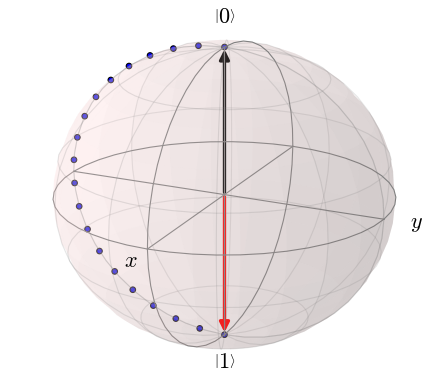
\includegraphics[width=0.75\textwidth]{img/blochxgate.png}
   \caption{Visualization of the X gate action on the Bloch sphere. The figure shows the X gate transforming the \0 state (black $+\hat{z}$-axis) into the \1 state (red $-\hat{z}$-axis) by means of an anti-clockwise $\pi$ rotation around the $\hat{x}$-axis.}
   \label{img:blochxgate}
\end{figure}

From Eq.~\ref{equ:xverification1},~\ref{equ:xverification2} and~\ref{equ:xverification3} it follows that X is its own inverse as well as its own Hermitian conjugate:
\begin{align}
XX &= XX^\dagger = \mathbb{1}\, , \\
X &= X^{-1} = X^\dagger\, .
\end{align}

Based on the textbook by \citeA{nielsen2010quantum}, the action, circuit \& matrix representation and Bloch sphere visualisation for some of the most important single-qubit quantum logic gates are summarised in Table~\ref{tab:singlequbitgates}.

\begin{table}[H]
\caption{Table of some major single-qubit quantum logic gates.}\vspace{0.15em}
\label{tab:singlequbitgates}
\begin{tabular}{ C{0.3cm}  C{2cm}  C{1.5cm}  C{1.5cm} C{2.5cm} C{2cm} C{3.5cm}}\hline
Gate & Name & Circuit representation & Matrix & Description & Rotation & Bloch sphere \\ \midrule
$\mathbb{1}$ & Identity & 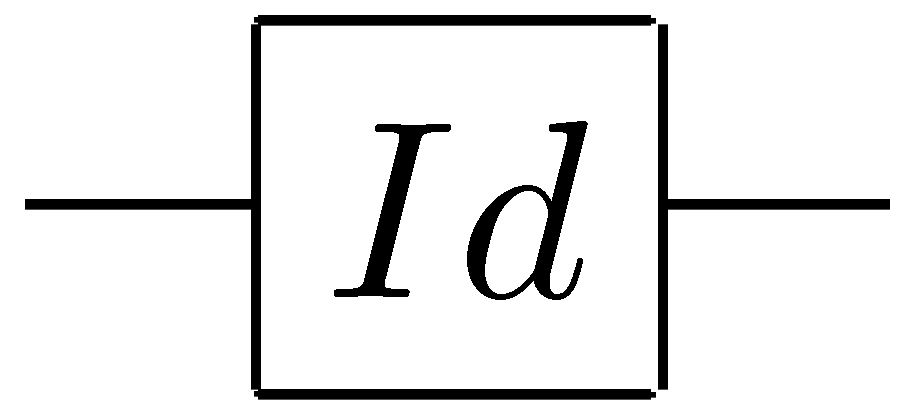
\includegraphics[width=0.1\textwidth]{img/identitycircuit.png} & $\begin{pmatrix}
 1 & 0 \\ 
 0 & 1
 \end{pmatrix}$ & Idle or waiting gate & - & - \\\midrule
X & Qubit flip & 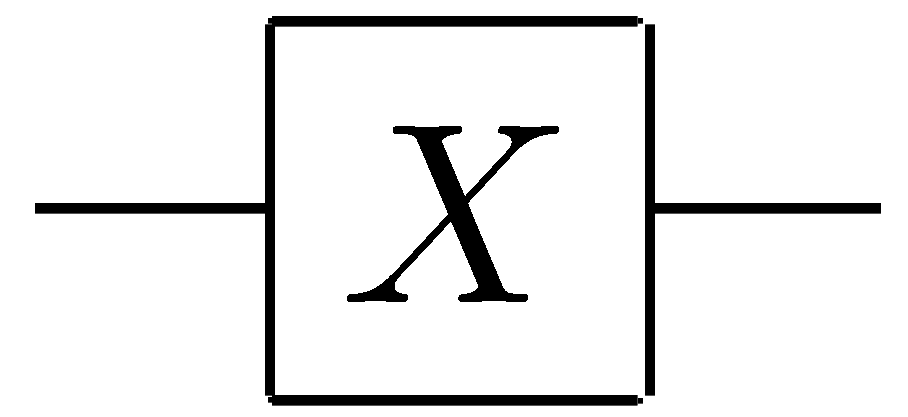
\includegraphics[width=0.1\textwidth]{img/xcircuit.png}  & $\begin{pmatrix}
 0 & 1 \\ 
 1 & 0
 \end{pmatrix}$ & Swaps amplitudes of \0 and \1 & $\pi$ rotation around $\hat{x}$ & 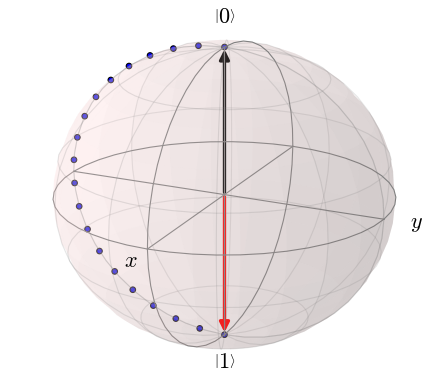
\includegraphics[width=0.2\textwidth]{img/blochxgate.png}\\\midrule
Y & Qubit \& phase flip & 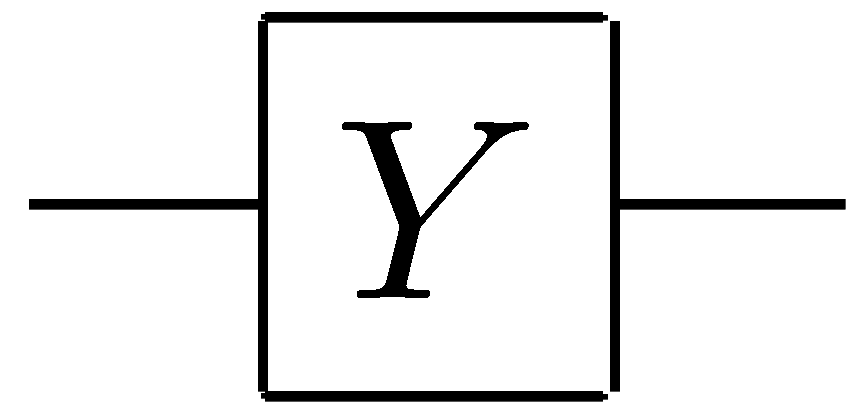
\includegraphics[width=0.1\textwidth]{img/ycircuit.png}  & $\begin{pmatrix}
 0 & -i \\ 
 i & 0
 \end{pmatrix}$ & Swaps amplitudes and introduces phase factor of $\pi$ (negative sign) to the \0 state & $\pi$ rotation around $\hat{y}$ &  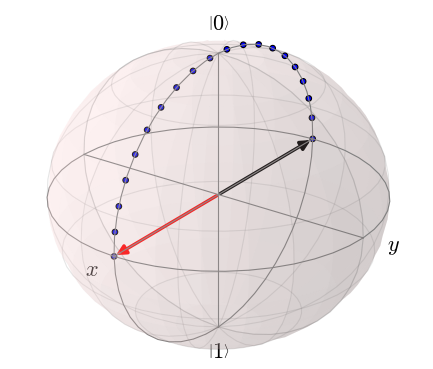
\includegraphics[width=0.2\textwidth]{img/blochygate.png}\\\midrule
Z & Phase flip & 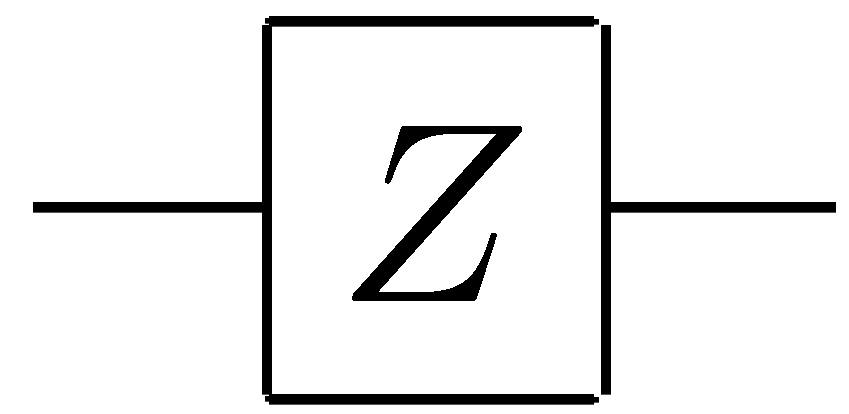
\includegraphics[width=0.1\textwidth]{img/zcircuit.png} & $\begin{pmatrix}
 1 & 0 \\ '
 0 & -1
 \end{pmatrix}$ & Introduces phase factor of $\pi$ (negative sign) to the \1 state & $\pi$ rotation around $\hat{z}$ & 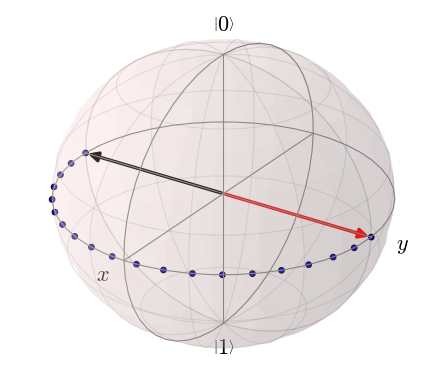
\includegraphics[width=0.2\textwidth]{img/blochzgate.png} \\\midrule 
H & Hadamard & 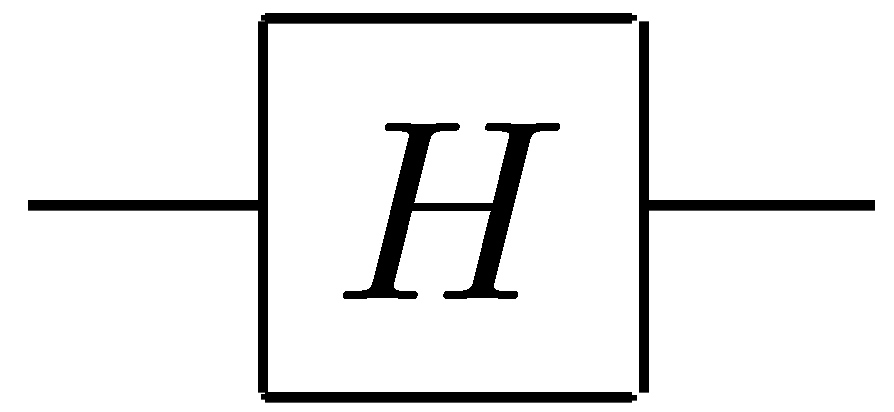
\includegraphics[width=0.1\textwidth]{img/hcircuit.png}  & $\begin{pmatrix}
 \frac{1}{\sqrt{2}} & \frac{1}{\sqrt{2}} \\ 
 \frac{1}{\sqrt{2}} & -\frac{1}{\sqrt{2}}
 \end{pmatrix}$ & Creates equal superposition & $\frac{\pi}{2}$ rotation around $\hat{y}$ and $\pi$ rotation around $\hat{x}$ & 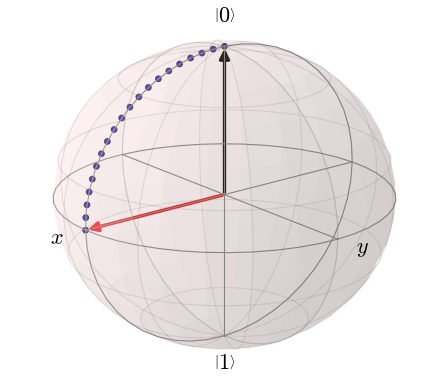
\includegraphics[width=0.2\textwidth]{img/blochhadamard.png}\\\midrule
S & $\frac{\pi}{2}$ rotation gate & 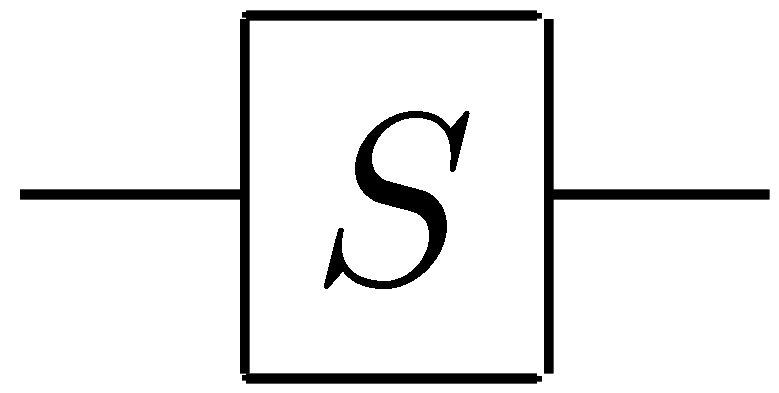
\includegraphics[width=0.1\textwidth]{img/scircuit.png} & $\begin{pmatrix}
 1 & 0 \\ 
 0 & i
 \end{pmatrix}$ & $\sqrt{Z}$ & $\frac{\pi}{2}$ rotation around $\hat{z}$ &  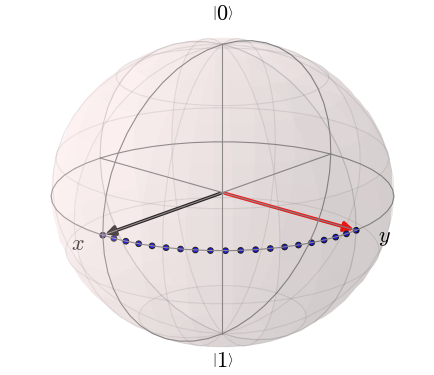
\includegraphics[width=0.2\textwidth]{img/blochsgate.png}\\\midrule
S$^\dagger$ & $-\frac{\pi}{2}$ rotation gate & 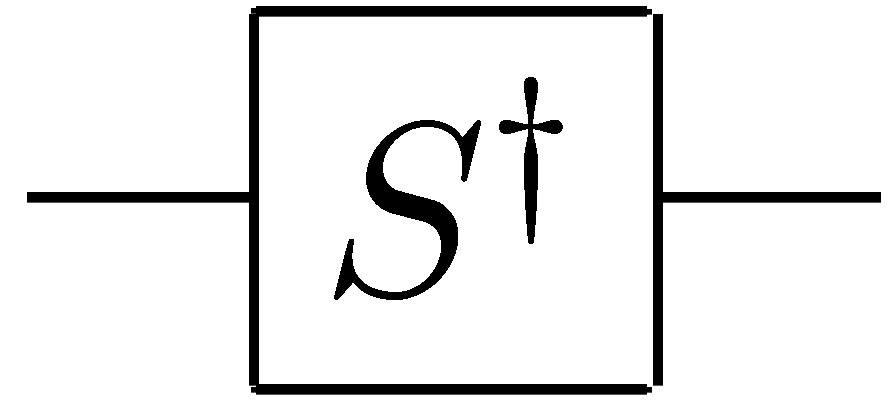
\includegraphics[width=0.1\textwidth]{img/sdcircuit.png} &  $\begin{pmatrix}
 1 & 0 \\ 
 0 & -i
 \end{pmatrix}$ & Hermitian conjugate of S & $-\frac{\pi}{2}$ rotation around $\hat{z}$ & \\\midrule
T & $\frac{\pi}{4}$ rotation gate & 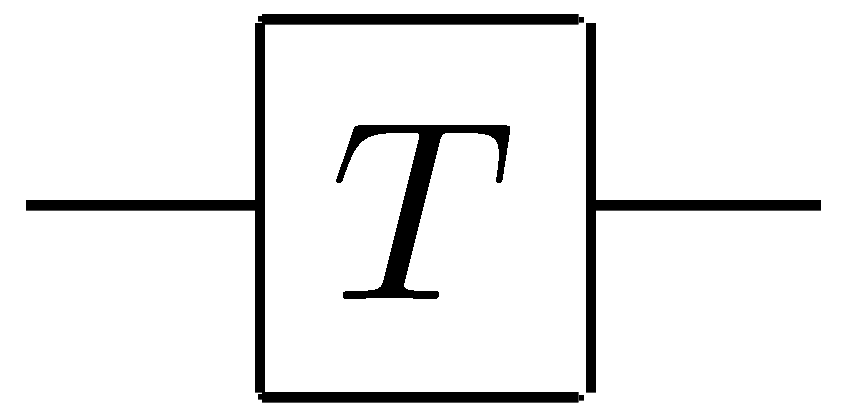
\includegraphics[width=0.1\textwidth]{img/tcircuit.png} & $\begin{pmatrix}
 1 & 0 \\ 
 0 & e^{\frac{i\pi}{4}}
 \end{pmatrix}$ & $\sqrt{S}$ & $\frac{\pi}{4}$ rotation around $\hat{z}$ & 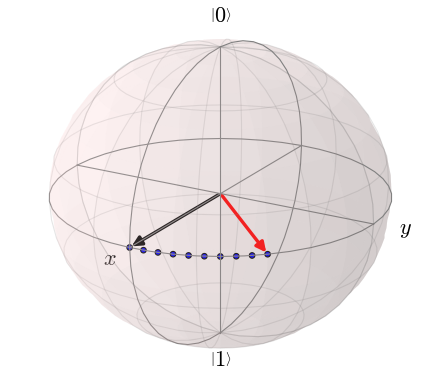
\includegraphics[width=0.2\textwidth]{img/blochtgate.png}\\\midrule
T$^\dagger$ & $-\frac{\pi}{4}$ rotation gate & 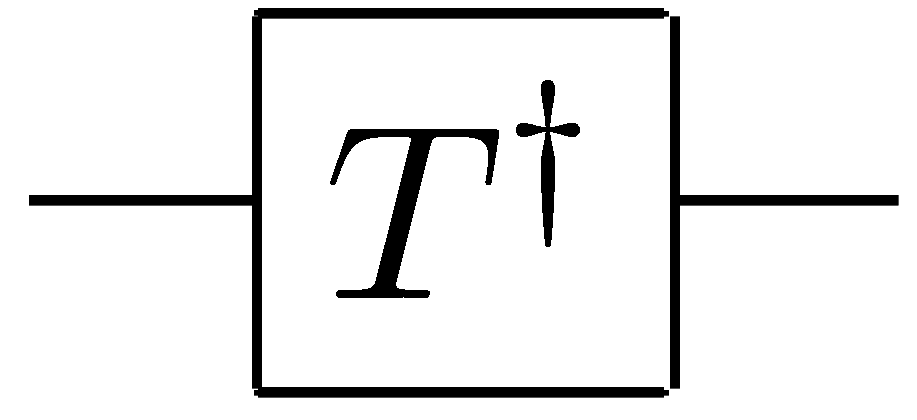
\includegraphics[width=0.1\textwidth]{img/tdcircuit.png} & $\begin{pmatrix}
 1 & 0 \\ 
 0 & e^{-\frac{i\pi}{4}}
 \end{pmatrix}$ & Hermitian conjugate of T & $-\frac{\pi}{4}$ rotation around $\hat{z}$ & \\\midrule
ZM & Z-basis measurement & 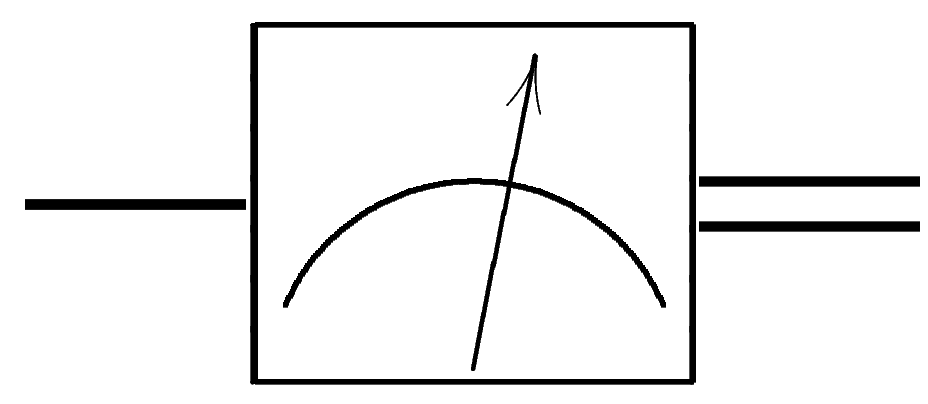
\includegraphics[width=0.1\textwidth]{img/measurecircuit.png} & - & Measurement in standard basis & Collapses the state & - \\
%\midrule
%BM & Bloch measurement & 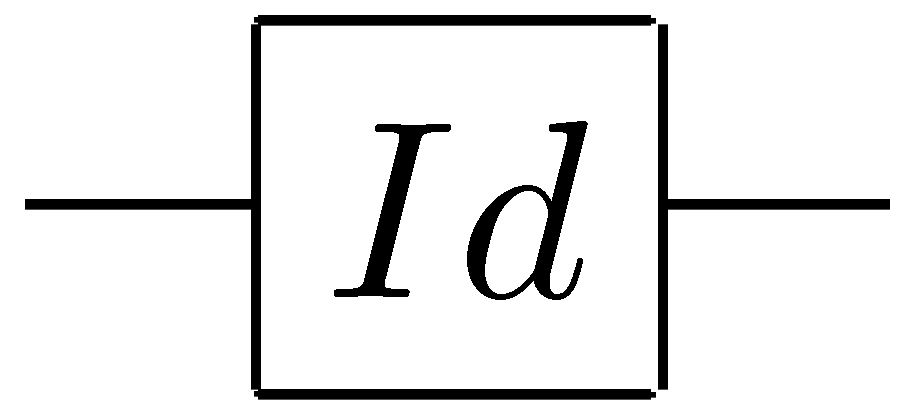
\includegraphics[width=0.1\textwidth]{img/identitycircuit.png} & - & Quantum state tomography & Collapses the state  & -\\
\end{tabular}
\end{table}


%%%%% SUBSECTION: MULTIPLE Q LOGIC GATES
\subsection{Multi-qubit gates}
\label{subsubsec:multiqubitgates}
\begin{table}[H]
\begin{center}
\begin{tabular}{l|lccc}\hline
Input & Output \\ \hline
00 & 00 \\
01 & 01 \\
10 & 11 \\
11 & 10 \\ \hline
\end{tabular}
\end{center}
\caption{Truth table for the CNOT quantum gate with the first qubit as control and the second qubit as target.}\vspace{1ex}
\label{tab:cnottruthtable}
\end{table}
%\subsubsection{Controlled-NOT gate}
%\label{subsubsubsec:cnotgate}
Multi-qubit quantum logic gates act on at least two qubits at the same time. Similar to single-qubit gates, an $n$-qubit quantum gate can be represented as a $2^n\times2^n$ unitary matrix. Since they involve multiple qubits, the Bloch sphere cannot longer be used to visualise their action. The two-qubit controlled NOT quantum gate will be used to demonstrate the properties, matrix representation and action of a two-qubit quantum gate. This can then easily be generalized to $n$-qubit quantum gates.

The controlled NOT or CNOT gate is given by the following $4\times4$ matrix:
\begin{equation}
\mathrm{CNOT} \doteq \begin{pmatrix}
 \mathbb{1} & 0 \\ 
 0 & X
 \end{pmatrix} = \begin{pmatrix}
 1 & 0 & 0 & 0 \\ 
 0 & 1 & 0 & 0 \\
 0 & 0 & 0 & 1 \\
 0 & 0 & 1 & 0 \\
 \end{pmatrix}\, .
\end{equation}

The CNOT gate takes two qubits, a control and a target qubit, as input. If and only if the control qubit is in the \1 state, the NOT (X) quantum gate is applied to the target qubit. In equations, the CNOT will always be followed by parentheses containing the control (c) qubit followed by the target (t) qubit: CNOT(c,t). The input-output relation, called truth table, for the CNOT gate is given in Table~\ref{tab:cnottruthtable} at the top of the page.

To demonstrate the usefulness of the CNOT gate consider starting with two unentangled qubits both in the \0 state,
\begin{equation}
\ket{\phi_0} = \ket{0} \otimes \ket{0} = \ket{00}\, .
\end{equation}
Applying the H gate onto the first qubit yields the following (still unentangled) state:
\begin{equation}
\ket{\phi_1} = (H \otimes \mathbb{1}) \ket{\phi_0} = (H \otimes \mathbb{1}) \ket{00} = \frac{1}{\sqrt{2}} \ket{00} + \frac{1}{\sqrt{2}} \ket{10}\, .
\end{equation}
Now consider applying the CNOT gate to the state $\ket{\phi_1}$ whereby the control qubit is coloured in \textcolor{red}{red} and the target qubit is coloured in \textcolor{emerald}{green}:

\begin{equation}
\label{equ:cnotexamples}
CNOT(\textcolor{red}{0},\textcolor{emerald}{1}) (\frac{1}{\sqrt{2}} \ket{\textcolor{red}{0}\textcolor{emerald}{0}} + \frac{1}{\sqrt{2}} \ket{\textcolor{red}{1}\textcolor{emerald}{0}}) = \frac{1}{\sqrt{2}} \ket{\textcolor{red}{0}\textcolor{emerald}{0}} + \frac{1}{\sqrt{2}} (\textcolor{red}{\mathbb{1}} \otimes \textcolor{emerald}{X}) \ket{\textcolor{red}{1}\textcolor{emerald}{0}} = \frac{1}{\sqrt{2}} \ket{\textcolor{red}{0}\textcolor{emerald}{0}} + \frac{1}{\sqrt{2}} \ket{\textcolor{red}{1}\textcolor{emerald}{1}}\, .
\end{equation}
The last expression in Eq.~\ref{equ:cnotexamples} is one of the famous Bell states which are a set of four maximally entangled quantum states. Another Bell state was used in the entanglement example in Section~\ref{subsec:multiqubitsystems}. Thus, this example demonstrates how the CNOT gate is crucial for the generation of entangled states since it applies the X gate to a target qubit depending on the state of a second control qubit.
%was used as an example (Eq.~\ref{equ:2qubitnonfactorized}) for entanglement in Section~\ref{subsec:multiqubitsystems} and it 

The three most important multi-qubit quantum gates CNOT, Toffoli and nCNOT are characterised in Table~\ref{tab:multiqubitgates}.

\begin{table}[H]
\caption{Table containing some major multi-qubit quantum logic gates where $c_j$ stands for the j\textsuperscript{th} control qubit and $\mathbb{1}_k$ for the kxk identity matrix.}\vspace{1em}
\label{tab:multiqubitgates}
\begin{tabular}{ c  C{1.8cm}  C{2cm}  c C{3cm}}\hline
Gate & Name & Circuit representation & Matrix & Description \\ \midrule
CNOT & Controlled NOT & 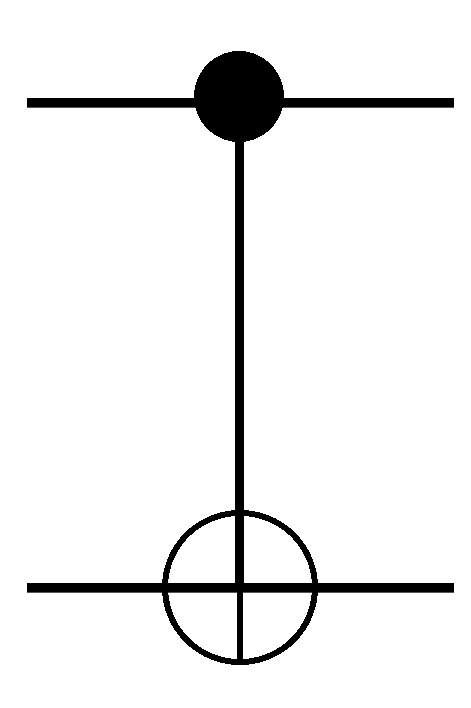
\includegraphics[width=0.1\textwidth]{img/cnotcircuit.png} & $\begin{pmatrix}
 \mathbb{1} & 0 \\ 
 0 & X
 \end{pmatrix} = \begin{pmatrix}
 1 & 0 & 0 & 0 \\ 
 0 & 1 & 0 & 0 \\
 0 & 0 & 0 & 1 \\
 0 & 0 & 1 & 0 \\
 \end{pmatrix}$ & CNOT($c_1$, target) \\\midrule
Toffoli & Controlled controlled NOT & 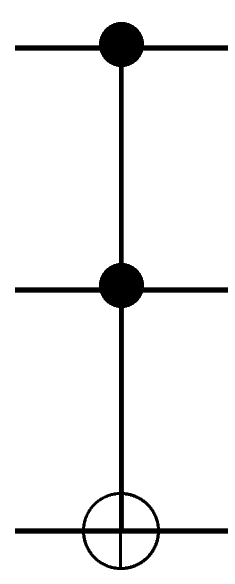
\includegraphics[width=0.1\textwidth]{img/ccnotcircuit.png}  & $\begin{pmatrix}
 \mathbb{1}_6 & 0 \\ 
 0 & X
 \end{pmatrix} = \begin{pmatrix}
 1 & 0 & 0 & 0 & 0 & 0 & 0 & 0 \\ 
 0 & 1 & 0 & 0 & 0 & 0 & 0 & 0 \\ 
 0 & 0 & 1 & 0 & 0 & 0 & 0 & 0 \\ 
 0 & 0 & 0 & 1 & 0 & 0 & 0 & 0 \\ 
 0 & 0 & 0 & 0 & 1 & 0 & 0 & 0 \\ 
 0 & 0 & 0 & 0 & 0 & 1 & 0 & 0 \\
 0 & 0 & 0 & 0 & 0 & 0 & 0 & 1 \\ 
 0 & 0 & 0 & 0 & 0 & 0 & 1 & 0 \\ 
 \end{pmatrix}$ & CCNOT($c_1$, $c_2$, target)\\\midrule
nCNOT & n-controlled NOT & -  & $\begin{pmatrix}
 \mathbb{1}_{2^n-2} & 0 \\ 
 0 & X
 \end{pmatrix}$ & nCNOT($c_1$,..,$c_n$, target) \\\midrule
\end{tabular}
\end{table}

%%%%% SECTION: MACHINE LEARNING

\section{Classical machine learning}
\label{subsec:classicalmachinelearning}

Machine learning (ML), a subfield of artificial intelligence, is aiming to enable computers to learn from data without a human explicitly programming its actions. It can be subdivided into the three major fields supervised \& unsupervised machine learning and reinforcement learning. The three areas can be most readily understood by considering the following three colloquial sentences:

\begin{redbox}
Supervised ML\\
- Based on \emph{input} and \emph{output} data\\
"I know how to classify this data, but I need an algorithm to do the computations for me."
\end{redbox}
\begin{greenbox}
Unsupervised ML\\
- Based on \emph{input} data only\\
"I have no clue how to classify this data, can the algorithm create a classifier for me?"
\end{greenbox}
\begin{bluebox}
Reinforcement learning\\
- Based on \emph{input} data only\\
"I have no clue how to classify this data, can the algorithm classify this data and I'll give it a reward if it's correct or I'll punish it if it's not."
\end{bluebox}

This thesis, specifically, is focusing on quantum-enhancements in the field of supervised machine learning only. The following section will introduce a well-known algorithm from the subfield of supervised ML: the $k$-nearest neighbour algorithm.

\subsection{Classical $k$-nearest neighbour algorithm}
\label{subsubsec:knearestneighbour}

Understanding the quantum version of the distance weighted $k$-nearest neighbour (kNN) algorithm as proposed by \citeA{Schuld2014} requires prior knowledge of the classical version of the algorithm that will be introduced in this subsection.

Imagine working for a search engine company and you are given the task of classifying unknown pictures of fruits as either apples or bananas. To train your classification algorithm, you are given five different pictures of apples and five different pictures of bananas. This will be called the \emph{training data set} ${D}_{T}$. The pictures in ${D}_{T}$ may be taken from various angles, in varying light settings and include different coloured apples and bananas. Two examples of such images are shown in Fig.~\ref{img:appleandbanana}. 

\begin{figure}[H]
  \begin{minipage}[t]{0.48\textwidth}
    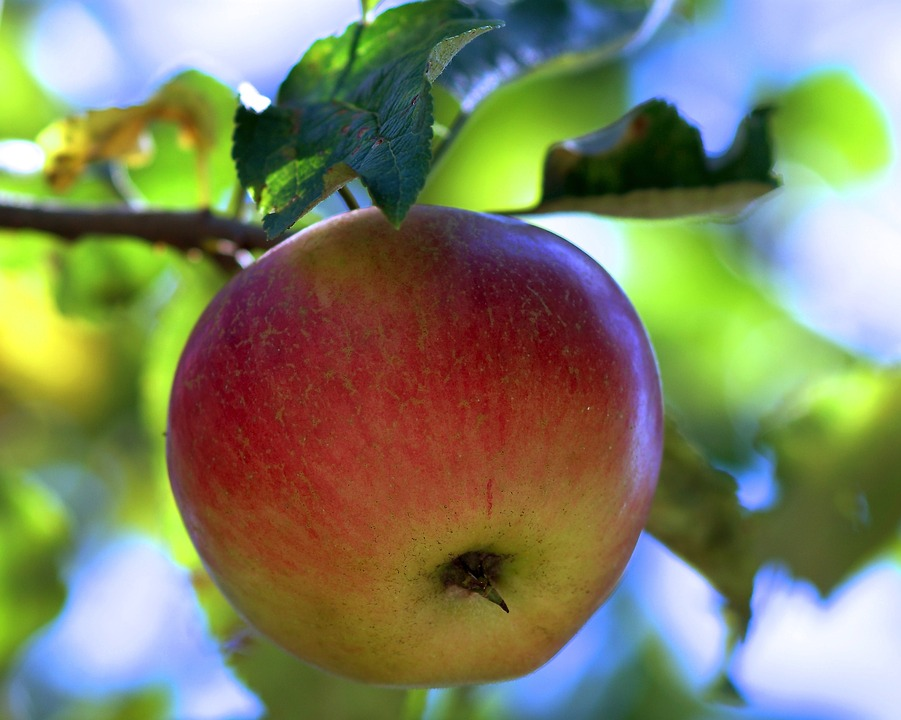
\includegraphics[width = \textwidth]{img/apple.jpg}
  \end{minipage}
  \hfill
  \begin{minipage}[t]{0.48\textwidth}
    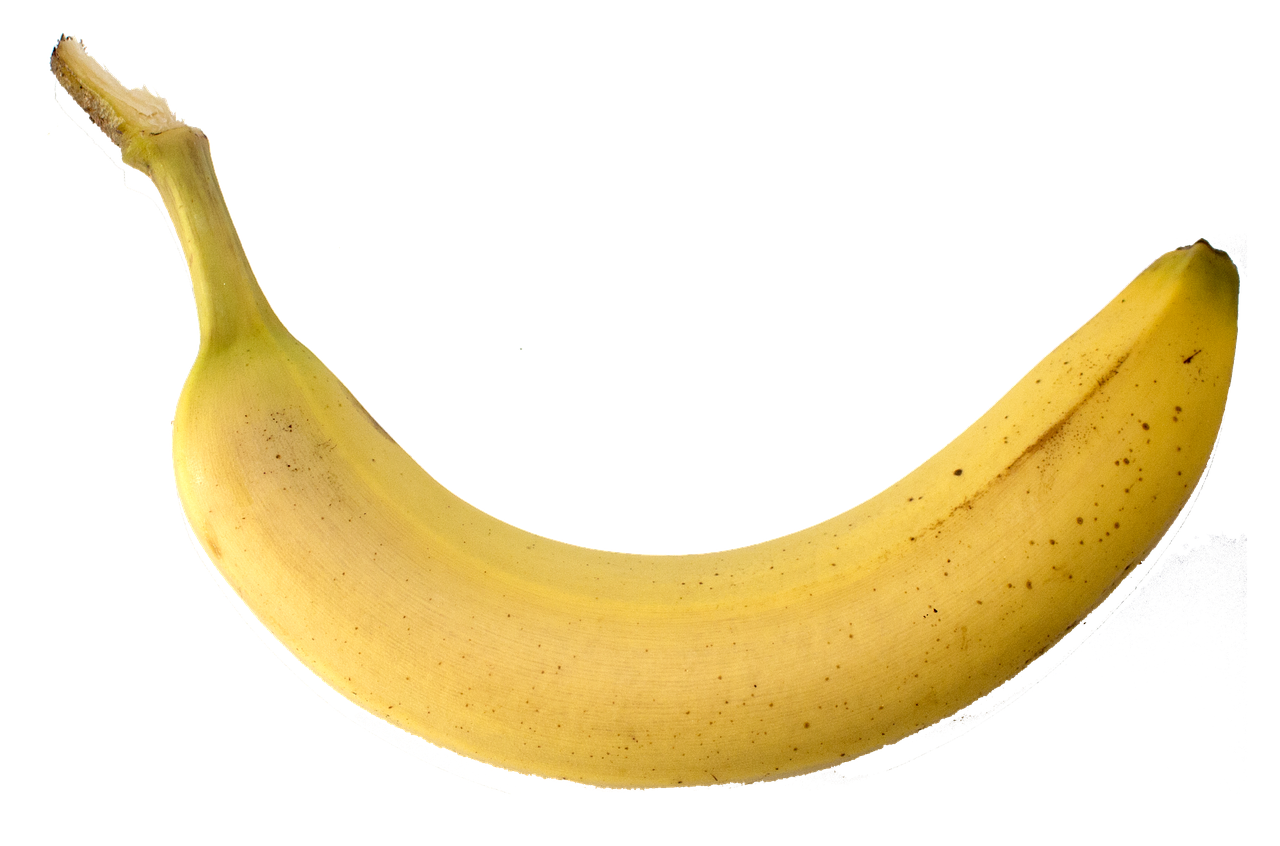
\includegraphics[width = \textwidth]{img/banana.png}
  \end{minipage}
  \caption[]{Pictures of apple and banana from training data set ${D}_{T}$.\footnotemark[3]}
  \label{img:appleandbanana}
\end{figure}

\footnotetext[3]{Reprinted from Pixabay, Retrieved December 24, 2016, from \url{https://pixabay.com/en/apple-red-fruit-frisch-vitamins-1632016/} and \url{https://pixabay.com/en/banana-fruit-yellow-1504956/}. Creative Commons Licence 2016 by Pixabay.}

Most of the time, using the full pixel representation of each picture for classification does not lead to optimal results. Therefore, the next step is to select a certain number of characteristic \emph{features} extracted from the pictures in the training set that can be used to differentiate apples from bananas. Such a feature might be the RGB value of the most frequent pixel colour since bananas and apples have different colour spectra. Using a measure of the curvature of the main object in the picture is another possibility since an apple is almost spherical whereas a banana looks more like a bend line.

By selecting and extracting features, the dimensionality of the training data set is drastically reduced from a few thousand pixels to a handful of features. The $m$ extracted features for the j\textsuperscript{th} picture are stored in the $m$-dimensional \emph{feature vector} $\vec{v}_{j}$. Mathematically, the training data set ${D}_{T}$ consists of ten feature vectors $\vec{v}_{0}, \vec{v}_{1},..,\vec{v}_{10}$ that are each assigned to either class $A$ (apple) or $B$ (banana). The training vectors are visualised as yellow and purple circles in Fig.~\ref{fig:knnconcept}.

Given a new picture of either a banana or an apple, you first extract the same $m$ features from it and store it in the input vector $\vec{x}$. From many algorithms, you decide to use the kNN algorithm since it is a non-parametric classifier meaning it makes no prior assumption about the class of the new picture. Given a new unclassified input vector $\vec{x}$ (red star in Fig.~\ref{fig:knnconcept}), the algorithm considers the $k$ nearest neighbours within the training set (using a predefined measure of distance) and classifies $\vec{x}$, based on a majority vote, as either $A$ or $B$. Thereby, $k$ is a positive integer, usually chosen to be small and its value determines the classification outcome. Namely, in the case $k = 3$ in Fig.~\ref{fig:knnconcept}, vector $\vec{x}$ will be classified as class B (purple) but in the case $k = 6$ it will be labelled class A (yellow).

\begin{figure}[H]
      \centering
       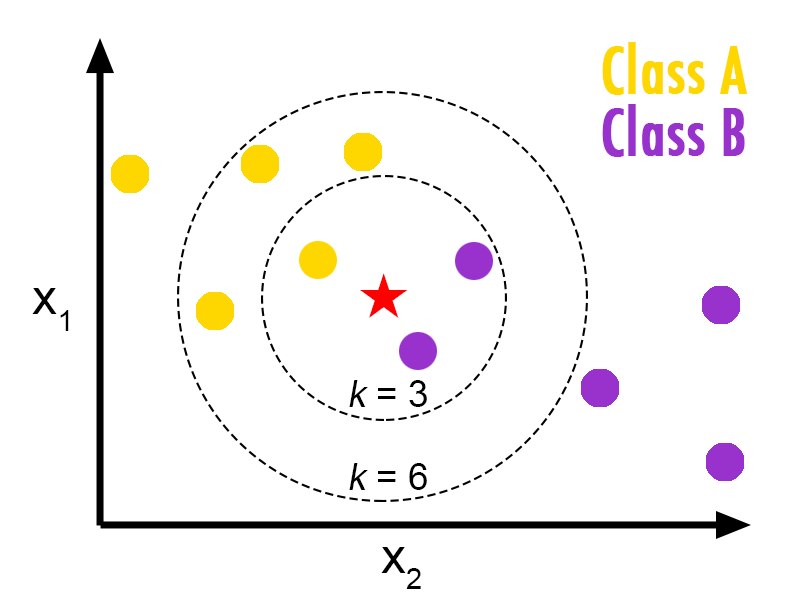
\includegraphics[scale=0.8]{img/knn-concept.png}
       \caption[]{\label{fig:knnconcept} Visualization of a kNN classifier\footnotemark[4]}
\end{figure}

\footnotetext[4]{Reprinted from GitHub, Burton de Wilde, Retrieved September 13, 2016, from \url{http://bdewilde.github.io/blog/blogger/2012/10/26/classification-of-hand-written-digits-3/}. Copyright 2012 by Burton de Wilde.}

In the case of $k = 10$, $\vec{x}$ would simply be assigned to the class with the most members. In this case, the training vectors should be given distance-dependent weights (such as $\frac{1}{distance}$) to increase the influence of closer vectors over more distant ones.

\subsection{Algorithmic time complexity: Big-O notation}
\label{subsubsec:algcomplexity}

%\subsubsection{Big-O notation}
%\label{subsubsubsec:bigO}
In the fields of computer science and quantum information, the so-called \emph{Big-O notation}, first described by \citeA{bachmann1894analytische}, is often used to describe how the runtime of an algorithm depends on variables such as the desired accuracy, the number of input vectors or their size. Hence, this is a way of quantifying the \emph{algorithmic time complexity} of a quantum algorithm. In the later sections of this thesis, the Big-O notation will be used as a tool to quantify possible quantum speed-ups in kNN quantum machine learning algorithms.

\begin{redbox}
\textbf{Definition: Big-O $\mathcal{O}$}\\
\newline
For any monotonic functions $t(n)$ and $g(n)$ defined on a subset of the real numbers (${\rm I\!R}$), one says that $t(n) = \mathcal{O}(g(n))$ if and only if when there exists constants $c \geq 0$ and $n_0 \geq 0$ such that

\begin{equation}
\mid t(n) \mid \quad \leq \quad c\text{ }\mid g(n) \mid\, , \quad \text{for all } n \geq n_0\, .
\end{equation}
\end{redbox}
\begin{redbox}
\begin{figure}[H]
      \centering
       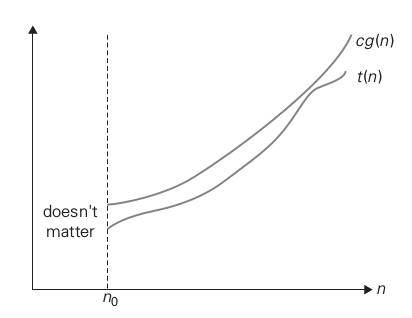
\includegraphics[scale=0.3]{img/asymptoticupperbound.png}
       \caption[]{\label{fig:upperasym} Visualization of $c\text{ }g(n)$ being an upper asymptotic bound for the function $t(n)$\footnotemark[5]}
\end{figure}

\footnotetext[5]{Reprinted from Anany Levitin and Soumen Mukherjee. Introduction to the Design \& Analysis of Algorithms. Reading, MA: Addison-Wesley, 2003. Copyright 2012 by Levitin \& Mukherjee.}

This implies that the function $t(n)$ does not grow at a faster rate than $g(n)$, or in other words that some constant multiple of the function $g(n)$ is an upper asymptotic bound for the function $t(n)$, for all $n\rightarrow \infty$.
\end{redbox}

Fig.~\ref{fig:algcomplexities} provides a good visual comparison between common algorithmic complexity classes regarding their relation to the input size $n$. It can be seen that the best possible algorithmic time complexity is constant time, $\mathcal{O}(1)$, that is being independent of the size of the input data e.g. determining if a binary number is even or odd. An algorithm is still considered excellent if it runs in logarithmic time $\mathcal{O}(log(n))$. Linear search algorithms, for example, are linear in time expressed as $\mathcal{O}(n)$. More complex sort algorithms like "bubble sort" have a higher time complexity and often run in quadratic time ($\mathcal{O}(n^2)$). Furthermore, algorithms with complexity $\mathcal{O}(n^c)$ are said to run in polynomial time for some $c > 2$. If an algorithm has time complexity $\mathcal{O}((log(n))^c)$ for some $c \geq 1$ it is called polylogarithmic. The highest complexity classes are exponential $\mathcal{O}(c^n)$ with $c \geq 1$ and factorial time $\mathcal{O}(n!)$. 
%For example, solving the travelling salesman problem using brute-force search runs in factorial time.

\begin{figure}[H]
      \centering
       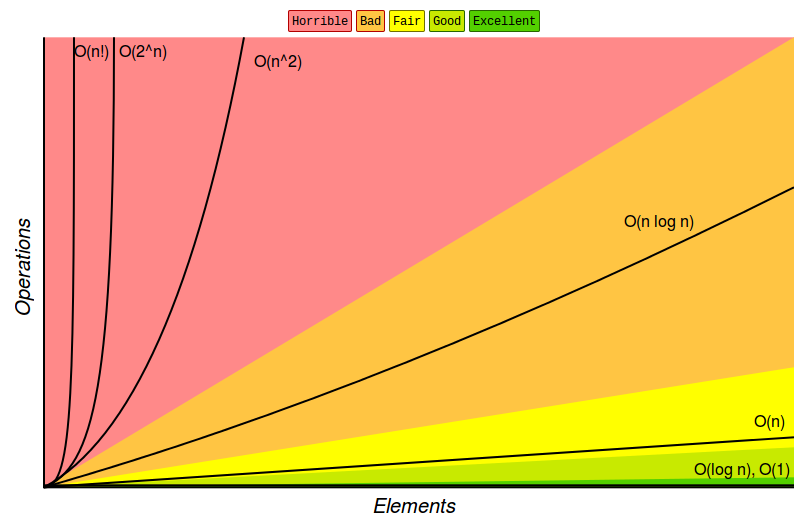
\includegraphics[scale=0.35]{img/bigocomplexity.png}
       \caption[]{\label{fig:algcomplexities} Overview of some major algorithmic complexity classes. In the figure, the number of operations (vertical axis) is plotted against the number of elements $n$ in the input data vector (horizontal axis). Based on colour coding defined on top of the table the following algorithmic time complexity classes are illustrated: constant time $\mathcal{O}(1)$, logarithmic time $\mathcal{O}(log(n))$, linear time $\mathcal{O}(n)$, linearithmic time $\mathcal{O}(n log(n))$, quadratic time $\mathcal{O}(n^2)$, exponential time $\mathcal{O}(2^n)$ and factorial time $\mathcal{O}(n!)$.\footnotemark[6]}
\end{figure}
\footnotetext[6]{Reprinted from Big-O Cheatsheet, Retrieved December 28, 2016, from \url{http://bigocheatsheet.com/}. Copyright 2016 by Big-O Cheatsheet.}

%TRANSITION TO NEXT SECTION NEEDED!
%\cleardoublepage
\chapter{Methods}\label{sec:methods}

The entirety of the research for this thesis is performed with pen and paper and a computer running the Linux operating system Ubuntu. The programming language Python, with its very intuitive syntax and extensive libraries for scientific computing and plotting, was used for the calculations and most of the plots for this thesis. More specifically, the open-source QuTiP library\footnotemark[7] for Python was used to create the Bloch sphere plots. All function plots were embedded directly into \LaTeX  by using the pgfplots package\footnotemark[8].

\footnotetext[7]{The open-source QuTiP library for Python may be downloaded from \url{http://qutip.org/}.}
\footnotetext[8]{The \LaTeX  pgfplots package may be downloaded from \url{https://www.ctan.org/pkg/pgfplots}.}

For the implementation of the quantum kNN algorithm, there are two fundamentally different ways: Running it a) by simulating a QC or b) by actually executing it on a real QC. The required tools for both possibilities will be explained in the following subsections.

\section{Liqui$\ket{}$}
\label{subsec:simulation}

Classical computers can be used to simulate the behaviour of small quantum computers. As outlined in Section~\ref{subsec:multiqubitsystems}, a QC with $n$ qubits can store the equivalent of $2^n$ classical bits in its $2^n$ amplitudes. It follows, that using a classical computer to simulate a QC with $n$ qubits requires storing all the $2^n$ amplitude values. Each amplitude has a complex and real part, hence, requiring two floating-point numbers to be stored. A floating-point number is encoded into 32 bits and storing each amplitude, thus, requires at least 64 classical bits of memory \cite{lambropoulos2007fundamentals}. As a result, a classical computer with at least $2^n\cdot64$ classical bits of random-access memory (RAM) is required to simulate an $n$-qubit quantum computer. As an example, only around two gigabytes (GB) of classical RAM are needed to simulate 25 qubits. Yet, the simulation of a QC with 44 qubits would require the world's fastest supercomputer Sunway TaihuLight with more than one petabyte of classical RAM \cite{chinasupercomputer}. Thus, simulating a quantum computer is associated with exponential computational costs thereby limiting the number of simulated qubits. Although, since current state-of-the-art quantum technology uses around ten qubits, a classical computer can still be used for simulation.

For the quantum computing simulations in this thesis the quantum simulation toolsuite Liqui$\ket{}$ developed by \citeA{liquid} will be used. Liqui$\ket{}$ is based on the functional programming language F\# and allows for simulation of up to 30 qubits \cite{microsoftresearch}. It comes with a large palette of predefined single and multi-qubit quantum logic gates and allows for custom-defined quantum gates such as nCNOT and rotation gates controlled by $n$ qubits which are crucial for some of the work done in this thesis. A short piece of example code from Liqui$\ket{}$ written in F\# is shown in Fig.~\ref{fig:liquidsnippet}. For all quantum simulations in this thesis, a Lenovo ThinkPad T450 with an Intel i5 processor (2 cores) and 8GB RAM is used.

\begin{figure}[H]
      \centering
       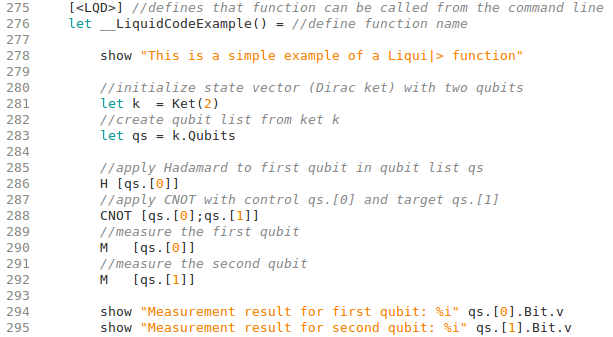
\includegraphics[scale=0.6]{img/liquidcodesnippet.png}
       \caption{\label{fig:liquidsnippet} F\# code snippet from Microsoft's quantum simulation toolsuite Liqui$\ket{}$. First, the code initialises two qubits in state $\ket{00}$ and applies an H gate to the first qubit leading to the state $\frac{\ket{00}+\ket{10}}{\sqrt{2}}$. Next, a CNOT gate, using the first and second qubit as control and target respectively, is applied. This leads to the maximally entangled state $\frac{\ket{00}+\ket{11}}{\sqrt{2}}$. Subsequently, both qubits are measured and the resulting bit values are displayed in the console.}
\end{figure}

\section{IBM Quantum Experience}
\label{subsec:ibmqc}

Since May 2016, IBM has enabled public cloud access to their experimental quantum processor containing five non-error-corrected superconducting qubits located at the IBM Quantum Lab at the Thomas J Watson Research Center in Yorktown Heights, New York \cite{ibmquantumcomputer}. Instead of only simulating on classical hardware, this opens up the possibility of executing the QML kNN algorithm on actual quantum hardware.

The so-called IBM Quantum Experience\footnotemark[9] provides the user with access to their \emph{quantum composer} which is the main tool for algorithm design. The quantum composer shown in Fig.~\ref{fig:composer} consists of 5 horizontal lines, one for each qubit, and enables the user to choose from a universal gate set (bottom of Fig.~\ref{fig:composer}) consisting of the following 10 quantum logic gates: $\mathbb{1}$, X, Y, Z, H, S, S$^\dagger$, T, T$^\dagger$ and CNOT. Additionally, there are two different types of measurement:
\begin{enumerate}[(a)]
\item A measurement in the standard basis, resulting in a probability distribution over the \0 and \1 state.
\item A Bloch measurement that visually projects the state onto the Bloch sphere. This is achieved by performing so-called \emph{quantum state tomography}\footnotemark[10] on the qubit while ignoring possible entanglement with other qubits \cite{ibmqetomo}.
\end{enumerate}
Through simple drag and drop the user can move any of those quantum logic and measurement gates into the quantum composer to create a quantum algorithm. However, the current version of the IBM Quantum Experience only allows the application of up to 40 quantum logic and measurement gates per qubit in the composer.
\footnotetext[9]{The IBM Quantum Experience can be accessed via \url{https://quantumexperience.ng.bluemix.net/qstage/}.}
\footnotetext[10]{A detailed explanation of quantum state tomography exceeds the scope of this thesis. The interested reader is referred to \citeA{altepeter649quantum}.}

\begin{figure}[H]
      \centering
       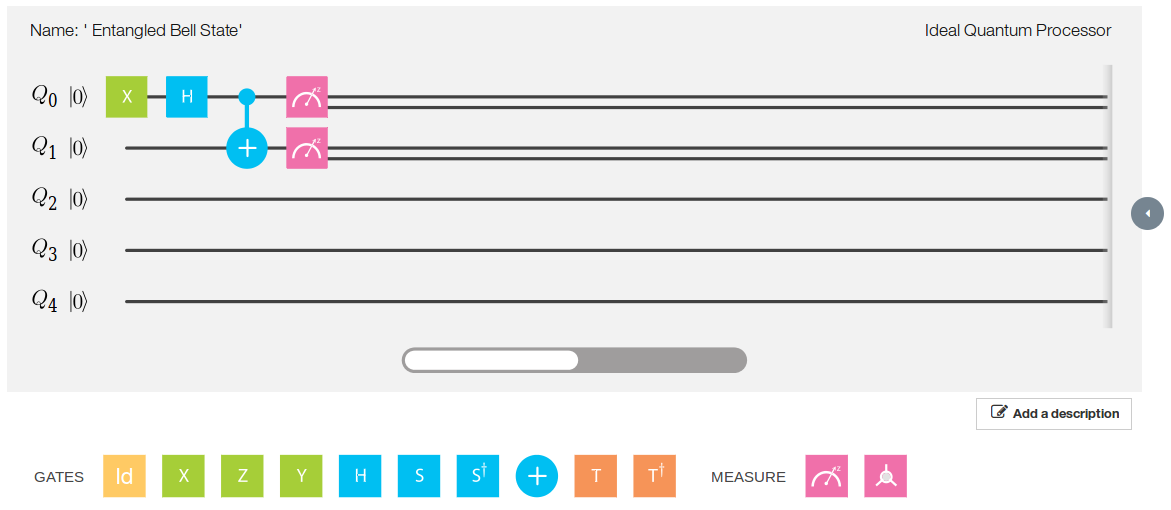
\includegraphics[scale=0.36]{img/ibmcomposer.png}
       \caption[]{\label{fig:composer} Screenshot showing the IBM Quantum Composer. For each of the five qubits $Q_0$,...,$Q_4$ there is a horizontal line with 40 available quantum gate slots. Quantum gates chosen from the universal gate set at the bottom can be dragged and dropped into the quantum composer to create a quantum algorithm.\footnotemark[11]}
\end{figure}
\footnotetext[11]{Screenshot was taken from \url{https://quantumexperience.ng.bluemix.net/qstage/#/editor}.}

After registration, each user receives a limited number of units that are required to execute algorithms on the real quantum processor. A minimum of three units is required to send the gate sequence of a composed algorithm to IBM's QC in New York. Then, depending on the waiting queue and the availability of the QC the results will be send back via email within a few minutes or days. The IBM Quantum Experience also allows for free quantum simulations under ideal or real conditions which provide a great tool for experimentation without spending user units.

The main limitation of the IBM Quantum Experience are the qubit decoherence times since they restrict the maximum number of possible operations before the qubits lose their quantum behaviour and their quantum information. Therefore, the number of quantum gates per qubit is currently limited to only 40 which essentially means 39 logic gates and one measurement gate. According to the qubit calibration results shown in Fig.~\ref{fig:calibration}, the amplitude damping times of the five qubits range from \SI{52.3}{\micro\second} to \SI{81.5}{\micro\second}. Furthermore, the phase damping times range from \SI{60.9}{\micro\second} to \SI{112.4}{\micro\second}. Currently, the implementation of a single qubit quantum logic gate takes 130ns and applying a CNOT gate takes 500ns \cite{ibmgatetimes}.

\begin{figure}[H]
      \centering
       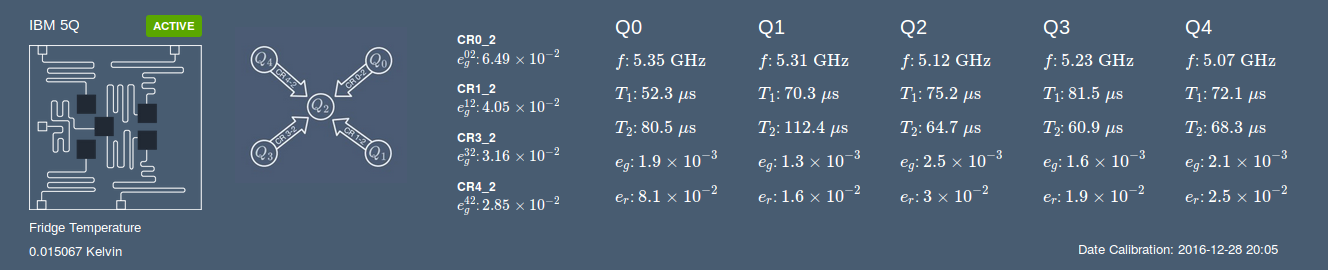
\includegraphics[scale=0.33]{img/ibmcalibration.png}
       \caption[]{\label{fig:calibration} Screenshot of IBM quantum processor calibration results showing the chip architecture, qubit arrangements, decoherence times and qubit error rates (28. December 2016 - 20:05).\footnotemark[12]}
\end{figure}
\footnotetext[12]{Screenshot was taken from \url{https://quantumexperience.ng.bluemix.net/qstage/#/editor}.}
%\cleardoublepage
\chapter{Literature Review: Quantum-enhanced Machine Learning}\label{sec:qml}

Classical machine learning takes classical data as input and learns from it using classical algorithms executed on classical computers - this will be referred to as C/C (classical data with classical algorithm). One enters the field of quantum machine learning when either quantum data or quantum algorithms are combined with ideas from classical machine learning. Thus, quantum machine learning can be subdivided into three different subfields: 1) C/Q - classical data with quantum algorithm, 2) Q/C - quantum data with classical algorithm and 3) Q/Q - quantum data with quantum algorithm.

\emph{Quantum data} includes any data describing a quantum mechanical system such as e.g. the Hamiltonian of a system or the state vector of a certain quantum state. A \emph{quantum algorithm} is any algorithm that can only be executed on a quantum computer. 

C/Q is the topic of this thesis

Analogously, Q/C is the subfield where quantum data is being processed using a classical machine learning algorithm. Examples for Q/C:

used genetic algorithms to reduce digi-
tal and experimental errors in quantum gates

A tantamount task is then to
find a model (a.k.a. effective) Hamiltonian of the system
and to determine properties of the present noise sources.
By computing likelihood functions in an adaptation of
Bayesian inference, Wiebe et al. found that quan-
tum Hamiltonian learning can be performed using realis-
tic resources such as depolarizing noise.

Q/Q would include learning a model Hamiltonian of a system implemented in a lab using a quantum learning algorithm.

\subsection{Quantum State Preparation Algorithms}
\label{subsubsec:quantumstatepreparation}

\emph{Quantum state preparation} is the process of preparing a quantum state that accurately represents a vector containing classical (normalized) data. There are two fundamentally different ways of preparing a quantum state representing the classical example vector v:

\begin{equation}
\label{equ:v}
v = \begin{pmatrix}0.6 \\ 0.4 \end{pmatrix}
\end{equation}

\subsubsection{Encoding classical data into qubits}
\label{subsubsec:classicaldataqubits}
%speed-up not very clear since the \# of qubits increases linearly with the \# of classical bits
The most straightforward type of quantum state preparation does not make use of quantum superpositions but only uses the definite \0 or \1 states to store binary information in a multi qubit system as outlined in the example below.

Multiply vector v by ten such that the normalized entries can easily be represented in binary,
\begin{equation}
\begin{pmatrix}
 \textcolor{blue}{0.6} \\ 
 \textcolor{emerald}{0.4}
 \end{pmatrix}*10 = \begin{pmatrix}
 \textcolor{blue}{6} \\ 
 \textcolor{emerald}{4}
 \end{pmatrix}
\end{equation}
 Convert each entry to binary,
 \begin{equation}
 \begin{pmatrix}
 \textcolor{blue}{6} \\ 
 \textcolor{emerald}{4}
 \end{pmatrix} \rightarrow \begin{pmatrix}
 \textcolor{blue}{0110} \\ 
 \textcolor{emerald}{0100}
 \end{pmatrix}
 \end{equation}

 Rewrite the 2-D vector as a 1-D bit string,
 \begin{equation}
 \begin{pmatrix}
 \textcolor{blue}{0110} \\ 
 \textcolor{emerald}{0100}
 \end{pmatrix} \rightarrow n=\textcolor{blue}{0110}\textcolor{emerald}{0100}
\end{equation}
For $g$ bits initialize $g$ qubits in the \0 state \& apply the X gate to the respective qubits:
\begin{equation}
n=\textcolor{blue}{0110}\textcolor{emerald}{0100}  \rightarrow \ket{n} = (\textcolor{blue}{\mathbb{1} \otimes X \otimes X \otimes \mathbb{1}}\otimes\textcolor{emerald}{\mathbb{1} \otimes X \otimes \mathbb{1} \otimes \mathbb{1}})\ket{00000000} = \ket{\textcolor{blue}{0110}\textcolor{emerald}{0100}}
\end{equation}
%\textbf{Only slight speed up possible}

When encoding classical data into qubit states, a $k$-dimensional probability vector requires $4k$ classical bits which are encoded one-to-one into $4k$ qubits. Thus, the number of qubits increases linearly with the size of the classical data vector. Due to this one-to-one correspondence between classical bits and qubits there is no data compression improvement compared to classical data storage. Only slight (up to quadratic) speed-ups are possible through clever quantum algorithm design (CITATION).

Qubit-based quantum state preparation becomes slightly more complicated when aiming to achieve a quantum memory state $\ket{M}$ in an equal superposition of $l$ binary patterns $l^j$ of the form

\begin{equation}
\label{equ:memorysuperpos}
\ket{M} = \frac{1}{\sqrt{l}}\sum^l_{j=1} \ket{l^j}
\text{where } \ket{l^j} = \ket{l^j_1,l^j_2,...l^j_n} \text{and } l^j_k \in \left\{0,1\right\}
\end{equation}

Preparing this quantum state is a requirement for the later used qubit-encoded kNN quantum algorithm by \citeA{Schuld2014}. \citeA{Trugenberger2001} describe a quantum routine that can efficiently prepare such a state as will be explained in detail below.

First, \citeA{Trugenberger2001} defines the new unitary quantum gate $S^j$,

\begin{equation}
S^j = \begin{pmatrix}
\sqrt{\frac{j-1}{j}} & \frac{1}{\sqrt{j}} \\
-\frac{1}{\sqrt{j}} & \sqrt{\frac{j-1}{j}}
\end{pmatrix}
\end{equation}

and introduces its controlled version $CS^j$:

\begin{equation}
CS^j = \begin{pmatrix}
\mathbb{1} & 0 \\
0 & S^j
\end{pmatrix}
\end{equation}

The initial quantum state is given in Equ.~\ref{equ:truginitial} and consists of three registers; the first being the pattern register containing the first pattern $l^1$, the second register $u$ is a utility register initialized in state $\ket{01}$ and the third register $m$ represents the memory register initialized with $n$ zeros in which all patterns $l^j$ will be loaded one after the other.

\begin{equation}
\label{equ:truginitial}
\ket{\Psi^1_0} = \ket{l^1;u;m} = \ket{l^1_1,l^1_1,...,l^1_n;01;0_1,...,0_n} 
\end{equation}

The routine will use the second utility qubit $u_2$ to separate the intial state into two terms whereby $u_2 = \ket{0}$ flags the already stored patterns and $u_2 = \ket{1}$ indicates the processing term. In order to store a pattern $l^j$ in the memory register one has to perform the following operations:

\begin{bluebox}
Step 1: Using $u_2$ as one of the control qubits for the CCNOT gate, copy the pattern $l^j$ into the memory register of the processing term ($u_2=\ket{1}$):
\begin{equation}
\label{equ:trug1}
\ket{\Psi^j_1} = \prod_{r=1}^n CCNOT(l^j_r,u_2,m_r)\ket{\Psi^j_0} 
\end{equation}

Step 2: If the qubits in the pattern and memory register are identical (true only for the processing term) then overwrite all qubits in the memory register with ones:
\begin{equation}
\label{equ:trug2}
\ket{\Psi^j_2} = \prod_{r=1}^n X(m_r)CNOT(l^j_r,m_r)\ket{\Psi^j_1} 
\end{equation}

Step 3: Apply a nCNOT gate controlled by all $n$ qubits in the $m$ register and flip $u_2$ if and only if all $n$ qubits are ones (true only for the processing term):
\begin{equation}
\label{equ:trug3}
\ket{\Psi^j_3} = nCNOT(m_1,m_2,...,m_n,u_2)\ket{\Psi^j_2} 
\end{equation}

Step 4: Using the previously defined $CS^j$ operation, with control $u_1$ and target $u_2$ , the new pattern is transferred from the processing term into the term containing the already stored patterns ($u_2 = \ket{0}$):
\begin{equation}
\label{equ:trug4}
\ket{\Psi^j_4} = CS^{l+1-j}(u_1,u_2) \ket{\Psi^j_3} 
\end{equation}

Step 5 \& 6: In Step 2 \& 3 all qubits in the memory register were overwritten with ones and these steps can be undone by applying their inverse operations:
\begin{align}
\label{equ:trug56}
\ket{\Psi^j_5} &= nCNOT(m_1,m_2,...,m_n,u_2)\ket{\Psi^j_4} \\
\ket{\Psi^j_6} &= \prod_{r=n}^1 CNOT(l^j_r,m_r)X(m_r)\ket{\Psi^j_5} 
\end{align}

The resulting state is now given by the following equation:

\begin{equation}
\label{equ:trug6}
\ket{\Psi^j_6} = \frac{1}{\sqrt{l}} \sum^{j}_{w=1} \ket{l^j;00;l^w} + \sqrt{\frac{l-j}{l}} \ket{l^j;01;l^j}
\end{equation}

Step 7: Finally, by applying the inverse operation of Step 1 the memory register of the processing term is restored to zeros only:
\begin{equation}
\label{equ:trug7}
\ket{\Psi^j_7} = \prod_{r=n}^1 CCNOT(l^j_r,u_2,m_r) \ket{\Psi^j_6} 
\end{equation}
\end{bluebox}

At the end of Step 7 the next pattern can be loaded into the first register and by applying Steps 1-7 again the pattern gets added to the memory register. After repeating this procedure $l$ times the memory register $m$ will be in the desired state $\ket{M}$ defined by Equ.~\ref{equ:memorysuperpos}.

\subsubsection{Encoding classical data into amplitudes}
\label{subsubsec:classicaldataamplitudes}

A more sophisticated way of representing the classical vector $v$ (Equ.~\ref{equ:v}) as a quantum state makes use of the large number of available amplitudes in a multi qubit system. The general idea is demonstrated in Equ.~\ref{equ:amplitudedata} below.

\begin{equation}
\label{equ:amplitudedata}
\begin{pmatrix}
 \textcolor{blue}{0.6} \\ 
 \textcolor{emerald}{0.4}
 \end{pmatrix} \quad \rightarrow \quad \ket{n} = \sqrt{\textcolor{blue}{0.6}}\ket{0}+\sqrt{\textcolor{emerald}{0.4}}\ket{1}
\end{equation}

Using amplitude-based quantum state preparation, a $k$-dimensional probability vector is encoded into only $log_{2}(k)$ qubits since the number of amplitudes grows exponentially with the number of qubits. This type of quantum data storage makes exponential compression of classical data possible. Since a quantum gate acts on all amplitudes in the superposition at once there is the possibility of exponential speed-ups in quantum algorithms compared to their classical counterparts. Compared to the one-to-one correspondence in qubit-encoded state preparation, amplitude-encoding requires a much smaller number of qubits that grows logarithmically with the size of the classical data vector. However, initializing an arbitrary amplitude distribution is still an active field of research and requires the implementation of non-trivial quantum algorithms.

For the case when the classical data vectors represent discrete probability distributions which are efficiently integrable on a classical computer, \citeA{Grover2002} developed a quantum routine to initialize the corresponding amplitude distribution.
%The main idea in their algorithm is subdividing the respective probability distribution and encoding the probabilty
%VERY COMPLICATED AND MOST GENERAL
Additionally, \citeA{soklakov2006efficient} proposed a quantum algorithm for the more general case that includes initializing amplitude distributions for classical data vectors representing non-efficiently integrable probability distributions.

\subsection{Quantum k-nearest Neighbour Algorithm}
\label{subsubsec:quantumknearestneighbour}

The quantum distance-weighted kNN algorithm outlined in this section was proposed by \citeA{Schuld2014} and is based on classical data being encoded into qubits rather than amplitudes. The first step is to prepare an equal superposition $\ket{T}$ over $N$ training vectors $\vec{v}$ of length $n$ with binary entries $v_1,v_2,...v_n$ each assigned to a class $c$ as follows,

\begin{equation}
\label{equ:qubitknninitial}
\ket{T} = \frac{1}{\sqrt{N}}\sum_{p=1}^N \ket{v_1^p,v_2^p,...v_n^p;c^p}
\end{equation}

The unknown vector $\vec{x}$ of length $n$ and binary entries $x_1,x_2,...x_n$ needs to be classified and is added to the training superposition resulting in the initial state $\ket{\psi_0}$:

\begin{equation}
\ket{\psi_0} = \frac{1}{\sqrt{N}}\sum_{p=1}^N \ket{x_1,x_2,...x_n;v_1^p,v_2^p,...v_n^p;c^p}
\end{equation}

An ancilla qubit initially in state \0 is added to the state such that the superposition is now described by,

\begin{equation}
\ket{\psi_1} = \frac{1}{\sqrt{N}}\sum_{p=1}^N \ket{x_1,x_2,...x_n;v_1^p,v_2^p,...v_n^p;c^p} \otimes \ket{0}
\end{equation}

The state now consists of four registers: 1) input($x$) register, 2) training($v$) register, 3) class($c$) register and 4) ancilla($\ket{0}$) register. Next, the ancilla register is put into an equal superposition by applying an H gate to it,

\begin{align}
\ket{\psi_2} &= \frac{1}{\sqrt{N}}\sum_{p=1}^N \ket{x_1,x_2,...x_n;v_1^p,v_2^p,...v_n^p;c^p} \otimes H\ket{0}\notag\\
&= \frac{1}{\sqrt{N}}\sum_{p=1}^N \ket{x_1,x_2,...x_n;v_1^p,v_2^p,...v_n^p;c^p} \otimes \frac{(\ket{0}+\ket{1})}{\sqrt{2}}
\end{align}

The main step in any kNN algorithm is calculating some measure of distance between each training vector $\vec{v}$ and the input vector $\vec{x}$ which in this quantum algorithm is taken to be the Hamming distance defined in the red box below.

\begin{redbox}
\textbf{Hamming distance (CITATION?)}\\
\newline
Hamming distance (HD) is the number of differing characters when comparing two equally long binary patterns $p_0$ and $p_1$.\\
\newline
Example:\\
$p_0 = \quad\textcolor{red}{0}\quad\textcolor{green}{0\quad1}$\\
$p_1 = \quad\textcolor{red}{1}\quad\textcolor{green}{0\quad1}$\\
$--------$\\
HD $= 1+0+0 = 1$
\end{redbox}

Given quantum state $\ket{\psi_2}$ the HD between the input and each training register can be calculated by applying CNOT($x_s,v_s^p$) gates to all qubits in the first and second register using the input vector qubits $x_s$ as controls and the training vector qubits $v_s^p$ as targets. This will change the qubits in the second register according to the rules specified in Equ.~\ref{equ:distancerules}. 

\begin{equation}
\label{equ:distancerules}
d^p_s =
    \begin{cases}
      0, & \text{if}\ \ket{v_s^p} = \ket{x_s} \\
      1, & \text{otherwise}
    \end{cases}
\end{equation}

The sum of the qubits in the second register now represents the total HD between each training register and the input. Applying an X gate to each qubit in the second register reverses the HD such that small HDs become large and vice versa. This is crucial since training vectors close to the input should get larger weights than more distant vectors. The quantum state is now given by,

\begin{align}
\ket{\psi_3} &= \prod_{s=1}^n X(v^p_s)CNOT(x_s,v^p_s)\ket{\psi_2}\notag\\
&= \frac{1}{\sqrt{N}}\sum_{p=1}^N \ket{x_1,x_2,...x_n;d_1^p,d_2^p,...d_n^p;c^p} \otimes \frac{(\ket{0}+\ket{1})}{\sqrt{2}}
\end{align}

By applying the unitary operator $U$ defined by,

\begin{equation}
\label{equ:sumoperator}
U = e^{-i\frac{\pi}{2n}K}
\end{equation}

where

\begin{equation}
\label{equ:sumoperator}
K = \mathbb{1} \otimes \sum_s (\frac{\sigma_z+1}{2})_{d_s} \otimes \mathbb{1} \otimes (\sigma_z)_c
\end{equation}

the sum over the second register is computed. As a result, the total reverse HD, denoted $d_H(\vec{x},\vec{v}^p)$, between the $p$th training vector $\vec{v}^p$ and the input vector $\vec{x}$ is written into the complex phase of the p$th$ term in the superposition. The ancilla register is now separating the superposition into two terms due to a sign difference in the amplitudes (negative sign when ancilla is \1). The result is given by, 

\begin{align}
\ket{\psi_4} &= U\ket{\psi_3}\notag\\
&= \frac{1}{\sqrt{2N}}\sum_p^N e^{i\frac{\pi}{2n}d_H(\vec{x},\vec{v}^p)} \ket{x_1,x_2,...x_n;d_1^p,d_2^p,...d_n^p;c^p;0} \notag\\
&\quad\quad\quad\quad\quad\quad + e^{-i\frac{\pi}{2n}d_H(\vec{x},\vec{v}^p)} \ket{x_1,x_2,...x_n;d_1^p,d_2^p,...d_n^p;c^p;1}
\end{align}

Applying an H gate to the ancilla register transfers the $d_H(\vec{x},\vec{v}^p)$ from the phases into the amplitudes such that the new quantum state is described by,

\begin{align}
\label{equ:beforecm}
\ket{\psi_5} &= (\mathbb{1} \otimes \mathbb{1} \otimes \mathbb{1} \otimes H)\ket{\psi_4}\notag\\
&= \frac{1}{\sqrt{N}}\sum_p^N cos\big[\frac{\pi}{2n}d_H(\vec{x},\vec{v}^p)\big] \ket{x_1,x_2,...x_n;d_1^p,d_2^p,...d_n^p;c^p;0} \notag\\
&\quad\quad\quad\quad\quad\quad + sin\big[\frac{\pi}{2n}d_H(\vec{x},\vec{v}^p)\big] \ket{x_1,x_2,...x_n;d_1^p,d_2^p,...d_n^p;c^p;1}
\end{align}

At this point the ancilla qubit is measured along the standard basis and all previous steps have to be repeated until the ancilla is measured in the \0 state. Since it is conditioned on a particular outcome, this type of measurement is called \emph{conditional measurement} (CM). The probability of a successful CM is given by the square of the absolute value of the amplitude and is dependent on the average reverse HD between all training vectors and the input vector:

\begin{equation}
Prob(\ket{a} = \ket{0}) = \sum_p^N cos^2\big[\frac{\pi}{2n}d_H(\vec{x},\vec{v}^p)\big]
\end{equation}

Finally, to classify the input vector $\vec{x}$ the class register is measured along the standard basis. The probability of measuring a specific class c is then given by the following expression:

\begin{equation}
\label{equ:classprobs}
Prob(c) = \frac{1}{NProb(\ket{a} = \ket{0})} \sum_{l \in c} cos^2\big[\frac{\pi}{2n}d_H(\vec{x},\vec{v}^l)\big]
\end{equation}

%When rewriting Equ.~\ref{equ:beforecm} into the following form,

%\begin{align}
%\label{equ:beforecm2}
%\ket{\psi_5} &= \frac{1}{\sqrt{N}}\sum_{c=1}^d \ket{c} \otimes \sum_{l \in c} cos\big[\frac{\pi}{2n}d_H(\vec{x},\vec{v}^l)\big] \ket{x_1^l,x_2^l,...x_n^l;d_1^l,d_2^l,...d_n^l;0} \notag\\
%&\quad\quad\quad\quad\quad\quad\quad\quad\quad\quad + sin\big[\frac{\pi}{2n}d_H(\vec{x},\vec{v}^l)\big] \ket{x_1^l,x_2^l,...x_n^l;d_1^l,d_2^l,...d_n^l;1}
%\end{align}

%where $l$ runs over all vectors $\vec{v}$ of a particular class c.

From Equ.~\ref{equ:classprobs} it is evident that the probability of measuring a certain class $c$ is dependent on the average total reverse HD between all training vectors belonging to class $c$ and the input vector $\vec{x}$. Since the total reverse HD represent distance-dependent weights it gets clear why this is the quantum equivalent to a classical distance-weighted kNN algorithm.

In order to obtain a full picture of the probability distribution over the different classes a sufficient number of copies of $\ket{\psi_5}$ needs to be prepared and after successful CM on the ancilla qubit the class qubit needs to be measured.

\begin{redbox}
\textbf{Algorithmic complexity}\\
\newline
According to \citeA{Schuld2014}, the preparation of the superposition has a complexity of $\mathcal{O}(Pn)$ where $P$ is the number of training vectors and $n$ is the length of the feature vectors. The algorithm has to be repeated $T$ times in order to get a statistically precise picture of the results. Hence, the total quantum kNN algorithm has an algorithmic complexity of $\mathcal{O}(TPn)$. 
\end{redbox}


%\cleardoublepage
\chapter{Results and Discussion}\label{sec:resultsanddiscussion}


\subsubsection{Diffusion matrix from quantum random walks}
\label{subsubsubsec:diffusion}

For the simplest case, consider the entries in the classical probability vector v to be normal distributed, e.g.

CHECK THE ORDER!
\begin{equation}
v = \colvec{0.064180\\0.146860\\0.146770\\0.341590\\0.026840\\0.063590\\0.061700\\0.148470}
\end{equation}

The goal is to encode this classical data into a quantum memory state $\ket{M}$ of the form,

\begin{align}
\ket{M} = \quad &0.064180 \ket{000} +
0.146860 \ket{100} +
0.146770 \ket{010} +
0.341590 \ket{001}\notag\\
&+ 0.026840 \ket{110}
+ 0.063590 \ket{011} +
0.061700 \ket{101} +
0.148470 \ket{111}
\end{align}

%Before outlining how to prepare state $\ket{M}$ the notion of Hamming distance needs to be introduced.

Furthermore, a useful tool of visualizing the HDs between binary patterns made from three qubits is a 3-D cube as shown in Fig.~\ref{img:cubenoprobs}. On the cube, adjacent qubit patterns have a HD of 1 and the HD increases by 1 for every additional corner. For example, the qubit state $\ket{000}$ is adjacent to $\ket{100}$ since they only differ in one qubit ($HD=1$). Moving one more corner yields the state $\ket{101}$ or $\ket{110}$ which both have a HD of 2 compared to $\ket{000}$.

\begin{figure}[!ht]
       \centering
       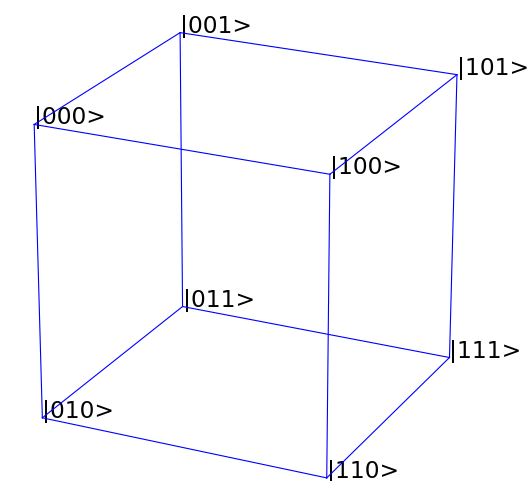
\includegraphics[width=0.5\textwidth]{img/cubewithoutprobs.png}
       \caption{\label{img:cubenoprobs} Visualizing Hamming distances on a 3-D cube}
\end{figure}

This way of visualizing HDs can be extended to the 16 binary patterns made by four qubits that can be visualized on a 4-D cube, also called tesseract, as illustrated in Fig.~\ref{img:hypercubenoprobs}.

\begin{figure}[!ht]
       \centering
       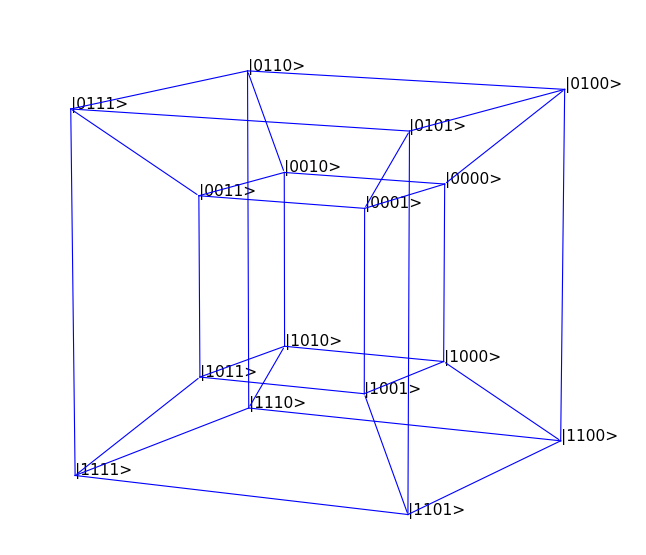
\includegraphics[width=0.5\textwidth]{img/hypercubewithoutprobs.png}
       \caption{\label{img:hypercubenoprobs} Visualizing Hamming distances on a 4-D cube (tesseract)}
\end{figure}

The idea of a coin operator $C$ can be borrowed from the theory of quantum random walks to initialize a gaussian distribution centered around a chosen binary qubit pattern. For this purpose, the coin operator is defined as,

\begin{equation}
C = \begin{pmatrix}
\sqrt{\delta} & 1-\sqrt{\delta} \\
1-\sqrt{\delta} & -\sqrt{\delta}
\end{pmatrix}
\end{equation}

where $0 \leq \delta \leq 1$.


\subsubsection{Amplitude-based quantum kNN algorithm}
\label{subsubsubsec:quantumknearestneighbouramplitudes}

\begin{equation}
\frac{1}{\sqrt{2M}}\sum_{m=1}^{M} (\textcolor{emerald}{\ket{0}}\ket{\textcolor{red}{\Psi_{\tilde{x}} (\star)}}+\textcolor{emerald}{\ket{1}}\ket{\textcolor{darkyellow}{\Psi}_{\textcolor{purple}{x^{m}}}})\ket{y^{m}(\textcolor{darkyellow}{A} \ or \ \textcolor{purple}{B})}\ket{m}
\end{equation}
where
\begin{equation}
\ket{\textcolor{red}{\Psi_{\tilde{x}} (\star)}} = \sum_{i=1}^{N} \textcolor{red}{\tilde{x}_i}\ket{i} \quad \quad
\ket{\textcolor{darkyellow}{\Psi}_{\textcolor{purple}{x^{m}}}}	 = \sum_{i=1}^{N} \textcolor{darkyellow}{x}\textcolor{purple}{_i^m} \ket{i} 
\end{equation}

\begin{equation}
e.g. \quad \begin{pmatrix}
 \textcolor{blue}{0.6} \\ 
 \textcolor{emerald}{0.4}
 \end{pmatrix} \quad \rightarrow \quad \ket{n} =  \sqrt{\textcolor{blue}{0.6}}\ket{0}+\sqrt{\textcolor{emerald}{0.4}}\ket{1}
\end{equation}

Applying the \textbf{Hadamard gate} interferes the input and the training vectors:

\begin{equation}
\frac{1}{2\sqrt{M}}\sum_{m=1}^{M} (\textcolor{emerald}{\ket{0}}[\ket{\textcolor{red}{\Psi_{\tilde{x}}}}+\ket{\textcolor{darkyellow}{\Psi}_{\textcolor{purple}{x^{m}}}}]+\textcolor{emerald}{\ket{1}}[\ket{\textcolor{red}{\Psi_{\tilde{x}}}}-\ket{\textcolor{darkyellow}{\Psi}_{\textcolor{purple}{x^{m}}}}])\ket{y^{m}(\textcolor{darkyellow}{A} \ or \ \textcolor{purple}{B})}\ket{m}
\end{equation}

$\rightarrow$ Perform \textbf{conditional measurement} on ancilla qubit.\\
Successful if $\ket{0}$ state is measured.

After successful conditional measurement, the state is proportional to
\begin{equation}
\frac{1}{2\sqrt{M}}\sum_{m=1}^{M} \sum_{i=1}^{N} (\textcolor{red}{\tilde{x}_i}+\textcolor{darkyellow}{x}\textcolor{purple}{_i^m})\ket{0}\ket{i}\ket{y^{m}(\textcolor{darkyellow}{A} \ or \ \textcolor{purple}{B})}\ket{m}
\end{equation}

Probability to measure class B:
\begin{equation}
p(\ket{y^m} = \ket{1(\textcolor{purple}{B})})= \sum_{m \mid y^m=1(\textcolor{purple}{B})} 1 - \frac{1}{4M} \mid \textcolor{red}{\tilde{x}} - \textcolor{purple}{x^m} \mid ^2
\end{equation}

Hereby, the advantages of the quantum version are the parallel computation of the distances between each training vector and the input vector as well as contracting distance computation and distance weighting into one computational step.

The quantum advantage of the algorithm is the simultaneous computation of the HD between the input vector and each training vector which is impossible to do classically. For example, if the training set contains 1,000,000 vectors with 10 entries each, the quantum algorithm performs all 1,000,000 distance computations with the application of only 10 X and 10 CNOT gates. In contrast, the classical algorithm would need to perform  1,000,000 individual computations in order to be able to apply distance-dependent weights to each training vector. 


\subsubsection{Controlled U Gate}
\label{subsubsubsec:controlledugate}

Often there is a need for applying certain quantum gates in a controlled manner. Thus a controlled U (CU) gate is required whereby U can be any unitary single-qubit gate. The CU gate is defined as:

\begin{equation}
CU = \begin{pmatrix}
 \mathbb{1} & 0 \\ 
 0 & U
 \end{pmatrix}
\end{equation}

It is important to note that the CNOT gate is essentially a CU gate in the case of U = X. 

Most of the time the CU gate cannot be implemented directly and has to be realized through larger quantum circuits consisting of CNOT and single-qubit gates. \citeA{nielsen2010quantum} describe such a decomposition as shown in Fig.~\ref{img:cudecomposition}.

\begin{figure}[ht]
   \centering
   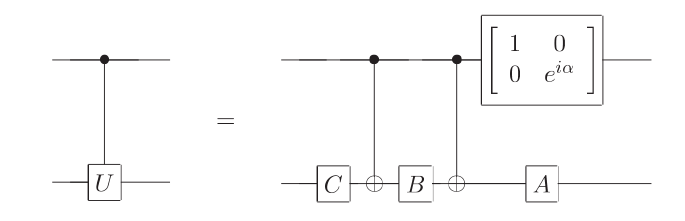
\includegraphics[width=0.7\textwidth]{img/controlledudecomp.png}
   \caption{Circuit decomposition for a controlled-U operation for single-qubit gate U.\textsuperscript{3}}
   \label{img:cudecomposition}
\end{figure}

\footnotetext[3]{Reprinted from Michael A. Nielsen and Isaac L. Chuang. Quantum Computation and Quantum Information. Cambridge University Press, 2000. Copyright 2010 by Nielsen \& Chuang.}

The idea is that when the control qubit is \0 the gate combination ABC is applied to the target qubit and has to equal the identity gate:

\begin{equation}
ABC = \mathbb{1}
\end{equation}

If and only if the control qubit is \1 then the gate sequence $e^{i\alpha}AXBXC$ is applied to the target. Since the goal is to apply the unitary U to the target qubit the following equation must be satified,

\begin{equation}
e^{i\alpha}AXBXC = U
\end{equation}

In order to find the matrices A,B,C and the additional parameter $\alpha$ the following equation has to be solved:

\begin{equation}
U = \begin{pmatrix}
 e^{i(\alpha-\frac{\beta}{2}-\frac{\delta}{2})}\cos{\frac{\gamma}{2}} & -e^{i(\alpha-\frac{\beta}{2}+\frac{\delta}{2})}\sin{\frac{\gamma}{2}} \\ 
e^{i(\alpha+\frac{\beta}{2}-\frac{\delta}{2})}\sin{\frac{\gamma}{2}} & e^{i(\alpha+\frac{\beta}{2}+\frac{\delta}{2})}\cos{\frac{\gamma}{2}}
 \end{pmatrix}
\end{equation}
%\cleardoublepage
\chapter{Outlook}\label{sec:outlook}
%\cleardoublepage
\chapter{Conclusion}\label{sec:conclusion}

Quantum-enhanced machine learning aims to harness the properties of quantum mechanical systems to enhance the performance of classical machine learning algorithms beyond the reach of classical computers. This becomes increasingly important since big data pushes computational resources and classical algorithms to their limits. This research established proof-of-principle simulations of two variants of a distance-weighted quantum $k$-nearest neighbour (kNN) algorithm using three small-scale supervised machine learning tasks.
%However, current quantum computing efforts have not yet led to the construction of a large-scale universal quantum computer and, thus, most of the current quantum-enhanced machine learning research is purely theoretical. Yet, small-scale quantum computers have been realised already and up to 30 qubits can still be simulated on a conventional laptop. Thus, this research is part of the attempt to shift quantum-enhanced machine learning into a more applied field by establishing proof-of-principle simulations of two variants of a distance-weighted quantum $k$-nearest neighbour (kNN) algorithm using three small-scale supervised machine learning tasks.
%On the other hand, IBM has enabled public access to their five-qubit quantum computer and small quantum computers with up to 30 qubits can still be simulated on conventional laptops. 

Firstly, the qubit-based kNN algorithm by \citeA{Schuld2014} was combined with a quantum state preparation routine by \citeA{Trugenberger2001} to classify various 9-bit RGB colours into the classes \emph{red} and \emph{blue}. Microsoft's software architecture Liqui$\ket{}$ was used to simulate the algorithm on two levels of difficulty. In the easy evaluation stage, the quantum kNN achieved a classification accuracy of 75\% which was subsequently raised to 100\% in the more challenging evaluation stage with a larger training dataset. These results show that the qubit-based kNN routine is a very effective classification algorithm concerning 9-bit RGB colours.

Aiming for an implementation with the IBM Quantum Experience, an amplitude-based kNN algorithm (aKNN) was developed by \citeA{SchuldFingerhuth}.  A simple binary Bloch vector classification tasks was considered to keep the requirements on the quantum hardware as small as possible. The necessary quantum compiling steps mapping the quantum state preparation routine and the aKNN algorithm to the IBM quantum hardware were outlined. For that particular classification task, it was shown that it could not be implemented within IBM's 40 quantum gate slots. Even though an implementation might be feasible using different datasets, the research demonstrated that there are cases which require relatively large gate sequences for implementation. As an alternative, the Bloch vector classification problem using the aKNN algorithm was simulated in Liqui$\ket{}$. The simulated algorithm led to the correct classification of two Bloch vectors. Lastly, the aKNN algorithm was simulated for the classification of discrete Gaussian distributions constituting a higher-dimensional classification problem using a slightly more advanced quantum state preparation routine. The simulated algorithm classified 83.3\% of various discrete Gaussian distributions correctly.

Overall, the Liqui$\ket{}$ quantum simulations clearly demonstrated the effectiveness of both quantum kNN algorithms. When combined with more general quantum state preparation routines, these algorithms bear the potential to speed up the processing of big data. Thus, a breakthrough in the development of a universal quantum computer would not solely constitute a major milestone in physics but most probably also revolutionise the field of machine learning.

%\cleardoublepage
\chapter{Personal Reflection}\label{sec:personalreflection}

Personally, this bachelor thesis research has been instructive and beneficial in many different ways. Most importantly, I have had the opportunity to dedicate my entire time to learn about the subject of quantum information and, specifically, quantum machine learning in detail. Since these subjects are not taught within the curriculum of the Maastricht Science Programme (MSP) it was especially amazing to challenge myself to these notoriously difficult subjects within the intersection of quantum physics and computer science. In doing so, I have learned more about the methods of theoretical physics and gained additional experience in scientific programming with Octave, Python and F\#. Without prior knowledge of F\#, I was able to learn how to simulate quantum computations and quantum machine learning algorithms using the quantum simulation toolsuite Liqui$\ket{}$. Furthermore, I was able to use the first cloud-based quantum computer, the so-called IBM Quantum Experience, publicly released in May 2016 by IBM.

Alongside my research, I had the possibility to attend many great lectures, seminars and three conferences which were all generously funded by the Centre for Quantum Technology. This enabled me to get to know many renowned scientists working in the fields of quantum information, quantum machine learning, open quantum systems, quantum optics and quantum cryptography. Furthermore, I was provided with the opportunity to present my research at the 4\textsuperscript{th} South African conference for quantum information processing, communication and control in Cape Town in late November 2016. This constituted a big step with respect to my academic career and a great way of putting my acquired presentation skills to practice.

However, in retrospective I feel that I could have been more productive in office by structuring my work days more diligently. For example, the first one and a half months were mostly spent on reading research paper and text books to acquire the theoretical foundation for my research and little time was used to practice F\# within the Liqui$\ket{}$ framework. A possible solution for the future would be to divide each day into two parts: e.g. spending the morning with reading papers and books and the afternoon on practical work and programming. Besides this, I feel like I should have communicated my progress more with my internal supervisor Dr. Birembaut at the MSP.

In conclusion, the bachelor thesis research has showed me the importance of interdisciplinarity since the field of quantum information requires the understanding of concepts in computer science as well as quantum mechanics. Fortunately, MSP's liberal education does not only focus on textbook exercises and lectures but mostly teaches us how to systematically approach unknown topics and tackle problems therein. It was great to see that this enabled me to venture into a previously unfamiliar field and learn the necessary skills to conduct meaningful research. The newly acquired skills will certainly be useful for my planned masters in the field of quantum information.

%During the thesis work, I realized that encountering problem after problem is at the core of research but that one can resolve most of them when just showing enough dedication.

%The Centre for Quantum Technology at the University of KwaZulu-Natal in South Africa has been a wonderful host for my Bachelor thesis research. My supervisor Prof. Francesco Petruccione has become a mentor and friend and provided me with great opportunities for personal and academic growth. Furthermore, my collaborator Maria Schuld has shared vasts amount of knowledge, tricks and ideas with me and has always been a great help during my research work. Alongside my research, I had the possibility to attend many great lectures, seminars and three conferences which were all generously funded by the Centre for Quantum Technology. This enabled me to get to know many renowned scientists working in the fields of quantum information, quantum machine learning, open quantum systems, quantum optics and quantum cryptography. Attending the Quantum Machine Learning Workshop at the Dolphin Coast in July 2016 provided me with a broad overview of the field of quantum machine learning and was the first time that I ever attended a scientific conference. In November 2016, I was provided with the opportunity to present my research at the 4\textsuperscript{th} South African conference for Quantum Information Processing, Communication and Control in Cape Town. This opened the possibility for a collaboration with an experimental research group in Israel working on quantum computation with trapped ions. In January 2017, I am invited to the NiTheP Chris Engelbrecht Quantum Machine Learning Summer School where I will give three workshop sessions on quantum machine learning using the Liqui$\ket{}$ framework and the IBM Quantum Experience.
%\cleardoublepage
%\chapter{Working with \LaTeX\ }\label{sec:working}
This chapter explains how to typeset some of the most common elements contained in a technical report using \LaTeX.

\section{Headings}
Your report can be structured using several different types of headings. Use the commands \texttt{\textbackslash chapter\{.\}}, \texttt{\textbackslash section\{.\}}, \texttt{\textbackslash subsection\{.\}}, and \texttt{\textbackslash subsubsection\{.\}}. Use the asterisk symbol \texttt{*} to suppress numbering of a certain heading if necessary, for example, \texttt{\textbackslash section*\{.\}}.

\section{References and Footnotes}\label{sec:references}
References to literature are included using the command \texttt{\textbackslash
cite\{.\}}. For example \cite{optreg,motsys}. Your references must be entered in the file \texttt{bibliography.bib}. Making changes or adding new references in the bibliography file can be done manually or by using specialized software such as \textit{JabRef} which is free of charge.
 
Cross-referencing within the text is easily done using \texttt{\textbackslash label\{.\}} and \texttt{\textbackslash ref\{.\}}. For example, this paragraph is part of chapter~\ref{sec:working}; more specifically section~\ref{sec:references} on page~\pageref{sec:references}. You will need to compile your document twice in order for the cross-referencing to be updated.

Footnotes\footnote{The use of footnotes is generally not recommended.} are added using the command \texttt{\textbackslash footnote\{.\}}, but try to avoid the used of footnotes altogether.

\section{Lists}\label{sec:lists}
Three types of list-environments are commonly used: \texttt{itemize}, \texttt{enumerate}, and \texttt{description}. The following example uses \texttt{itemize} to create a list without numbering
\begin{itemize}
  \item point one; and
  \item point two
\end{itemize}
created using
\begin{verbatim}
\begin{itemize}
  \item point one; and
  \item point two
\end{itemize}
\end{verbatim}

The following example uses \texttt{enumerate} to create a list with numbering
\begin{enumerate}
  \item point one; and
  \item point two
\end{enumerate}
created using
\begin{verbatim}
\begin{enumerate}
  \item point one; and
  \item point two
\end{enumerate}
\end{verbatim}

The following example uses \texttt{description} to create a list with custom text as bullet-points
\begin{description}
  \item[P1] point one; and
  \item[P2] point two
\end{description}
created using
\begin{verbatim}
\begin{description}
  \item[P1] point one; and
  \item[P2] point two
\end{description}
\end{verbatim}


\section{Tables}\label{sec:tables}
Table~\ref{tab:table} shows an example of a simple table-layout. Try to avoid vertical lines on tables. The Internet contains countless resources on how to create special elements and structures in tables such as cells spanning multiple rows, rotated text, sideways tables, justification of cell elements, etc.
\begin{table}[ht]
\begin{center}
\caption{Driving cycle data of ECE-15, EUDC, and NEDC.}\vspace{1ex}
\label{tab:table}
\begin{tabular}{llccc}\hline
Description & Unit & ECE & EUDC & NEDC \\ \hline
Duration & s & 780 & 400 & 1180 \\
Distance & km & 4.052 & 6.955 & 11.007 \\
Average velocity & km/h & 18.7 &  62.6 & 33.6 \\
Idle speed & \% & 36 & 10 & 27 \\ \hline
\end{tabular}
\end{center}
\end{table}

This table was created using
\begin{verbatim}
\begin{table}[ht]
\begin{center}
\caption{Driving cycle data of ECE-15, EUDC, and NEDC.}\vspace{1ex}
\label{tab:table}
\begin{tabular}{llccc}\hline
Description & Unit & ECE & EUDC & NEDC \\ \hline
Duration & s & 780 & 400 & 1180 \\
Distance & km & 4.052 & 6.955 & 11.007 \\
Average velocity & km/h & 18.7 &  62.6 & 33.6 \\
Idle speed & \% & 36 & 10 & 27 \\ \hline
\end{tabular}
\end{center}
\end{table}
\end{verbatim}
Table~\ref{tab:table_advanced} shows a more advanced version of Tab.~\ref{tab:table} using the \texttt{booktabs} package. Inspect the source code of this document to see how this was done.
\begin{table}[ht]
\begin{center}
\small
\caption{Driving cycle data of ECE-15, EUDC, and NEDC.}\vspace{1ex}
\label{tab:table_advanced}
\begin{tabular}{@{}lcccc@{}}\toprule[1.5pt]
& & \multicolumn{3}{c}{\bf Driving cycle}\\
\cmidrule{3-5}
Description & Unit & {ECE} & {EUDC} & {NEDC} \\ \midrule
Duration & \unit[]{s} & 780 & 400 & 1180 \\
Distance & \unit[]{km} & 4.052 & 6.955 & 11.007 \\
Average velocity & \unitfrac[]{km}{h} & 18.7 &  62.6 & 33.6 \\
Idle speed & \unit[]{\%} & 36 & 10 & 27 \\ \bottomrule[1.5pt]
\end{tabular}
\end{center}
\end{table}



\section{Working with Units}
The package \texttt{\textbackslash usepackage\{units\}} enables two useful commands, namely \texttt{\textbackslash unit[.]\{.\}} and \\ \texttt{\textbackslash unitfrac[.]\{.\}\{.\}}. Use these commands to display units in a concise way, for example
\begin{align}
\delta t &= \unit[1]{s}\\
v &= \unitfrac[5]{m}{s}.
\end{align}
This example was done using
\begin{verbatim}
\begin{align}
\delta t &= \unit[1]{s}\\
v &= \unitfrac[5]{m}{s}.
\end{align}
\end{verbatim}

\section{Including Graphics}\label{sec:epsgraph}
It is recommended that you only use encapsulated post-script graphics \texttt{.eps} in your report. If you mix \texttt{.eps} with other formats such as \texttt{.png}, \texttt{.jpeg} or \texttt{.gif}, you will most likely not be able to compile your report without errors. Note that figures created in \textsc{Matlab} are easily saved in \texttt{.eps} format.

The inclusion of a figure can be done in the following way:
\begin{verbatim}
\begin{figure}[ht]
   \centering
   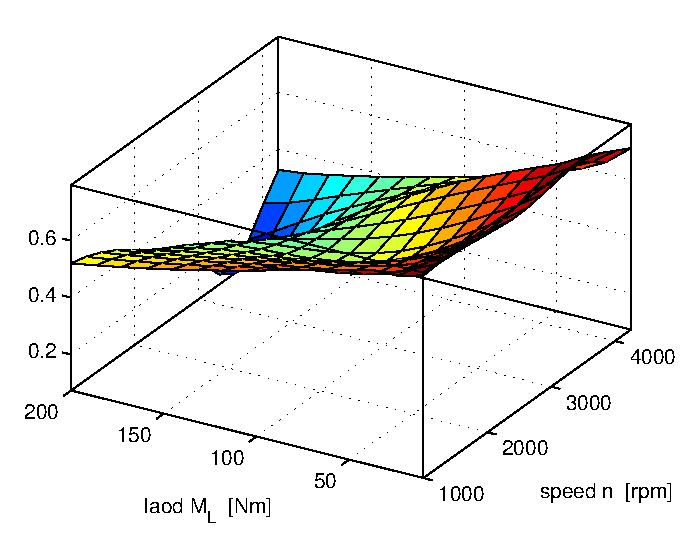
\includegraphics[width=0.75\textwidth]{img/k_surf.eps}
   \caption{Example of a figure.}
   \label{img:k_surf}
\end{figure}
\end{verbatim}

\begin{figure}[ht]
   \centering
   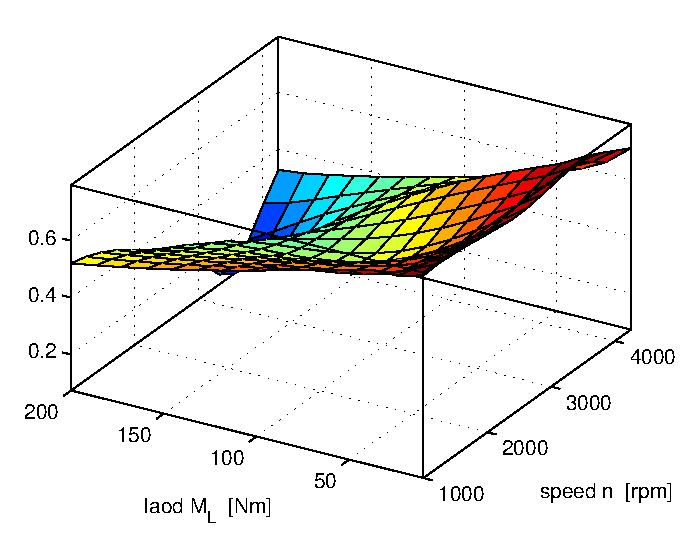
\includegraphics[width=0.75\textwidth]{img/k_surf.eps}
   \caption{Example of a figure.}
   \label{img:k_surf}
\end{figure}

Two figures are displayed next to each other using
\begin{verbatim}
\begin{figure}[ht]
  \begin{minipage}[t]{0.48\textwidth}
    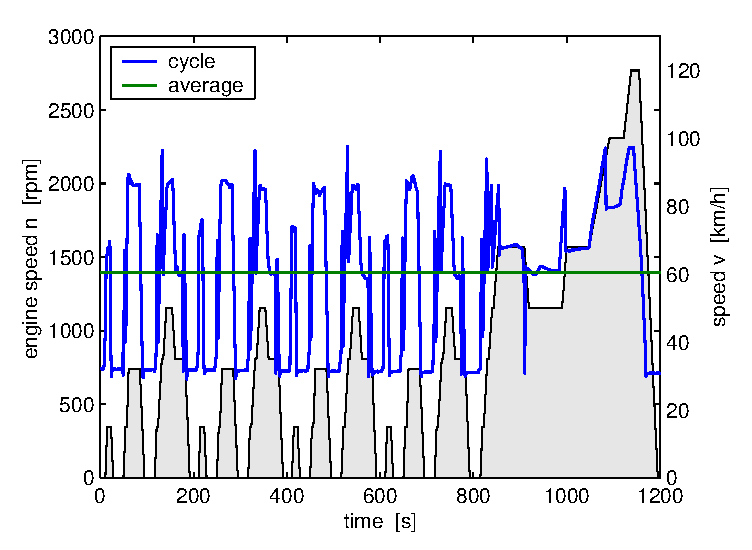
\includegraphics[width = \textwidth]{img/cycle_we.eps}
  \end{minipage}
  \hfill
  \begin{minipage}[t]{0.48\textwidth}
    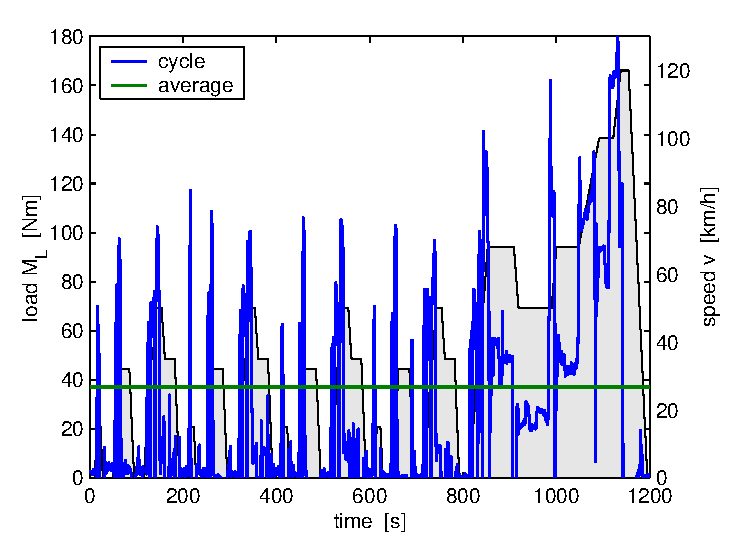
\includegraphics[width = \textwidth]{img/cycle_ml.eps}
  \end{minipage}
  \caption{Two figures next to each other.}
  \label{img:cycle}
\end{figure}
\end{verbatim}

\begin{figure}[ht]
  \begin{minipage}[t]{0.48\textwidth}
    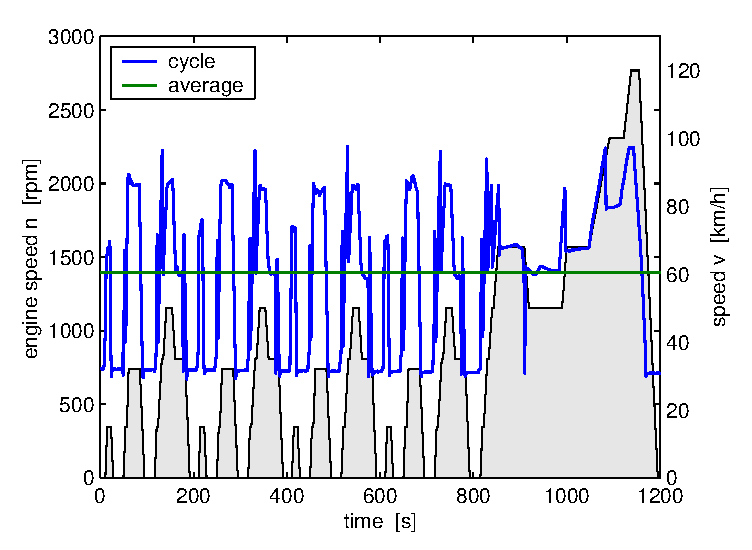
\includegraphics[width = \textwidth]{img/cycle_we.eps}
  \end{minipage}
  \hfill
  \begin{minipage}[t]{0.48\textwidth}
    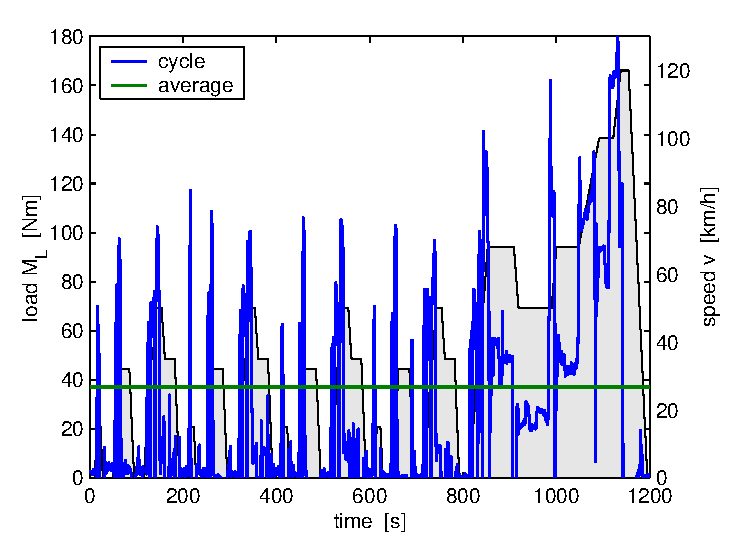
\includegraphics[width = \textwidth]{img/cycle_ml.eps}
  \end{minipage}
  \caption{Two figures next to each other.}
  \label{img:cycle}
\end{figure}

The positioning parameter \texttt{h} (here) forces your figure to be placed in the current position relative to your text. You may add \texttt{t} (top), \texttt{b} (bottom), and/or \texttt{p} (page) to allow for more flexible positioning within your document. For instance, \texttt{[tb]} forces your figure to be placed either on the top or bottom of a page.


\section{Equations}\label{sec:math}
The most common way to include equations is using the \texttt{equation} environment.
\begin{equation}\label{eq:p_me0f}
 p_\mathrm{me0f}(T_e,\omega_e) \ = \ k_1(T_e) \cdot (k_2+k_3 S^2
 \omega_e^2) \cdot \Pi_\mathrm{max} \cdot \sqrt{\frac{k_4}{B}} \, .
\end{equation}
It is recommended to use \texttt{\textbackslash mathrm\{.\}} for subscripts comprising more than two letters since it reduces the width of the subscript significantly and improves readability. The corresponding code is
\begin{verbatim}
\begin{equation}\label{eq:p_me0f}
 p_\mathrm{me0f}(T_e,\omega_e) \ = \ k_1(T_e) \cdot (k_2+k_3 S^2
 \omega_e^2) \cdot \Pi_\mathrm{max} \cdot \sqrt{\frac{k_4}{B}} \, .
\end{equation}
\end{verbatim}
Equations, such as Eq.~\eqref{eq:p_me0f}, may be referenced using \texttt{\textbackslash eqref\{.\}}. In-line mathematical content is created using \texttt{\$.\$}, for example $a^2+b^2=c^2$. It is practically possible to typeset any equation in \LaTeX. Equation~\eqref{eq:advanced} shows an example of a more advance structure.
\begin{equation}\label{eq:advanced}
x^k_n(i) = \left\{\begin{array}{ll}y(i) & \text{if}\quad x^k_{n-1}(i)\leq \mathbf{x}\\
z(i) & \text{otherwise}\end{array}\right., \text{for}\quad i=\{1,\ldots,N\}.
\end{equation}



\section{Including Code in your Document}
Include samples from your Matlab code using the \texttt{lstlistings} environment, for example
\lstset{language=Matlab,numbers=none}
\begin{lstlisting}[frame=lines]
% Evaluate y = 2x
for i = 1:length(x)

  y(i) = 2*x(i);

end
\end{lstlisting}
This example was created using
\begin{verbatim}
\lstset{language=Matlab,numbers=none}
\begin{lstlisting}[frame=lines]
% Evaluate y = 2x
for i = 1:length(x)

  y(i) = 2*x(i);

end
\end{lstlisting}
\end{verbatim}
where \texttt{\textbackslash usepackage\{mcode\}} must be included in the preamble of your document. If you want to include the entire content of a file \texttt{mycode.m} in your document, simply input the path to \texttt{mycode.m} instead of pasting the entire content into your \TeX -file
\begin{verbatim}
\lstset{language=Matlab,numbers=left}
\lstinputlisting{path/to/mycode.m}
\end{verbatim}
Including the path to your m-file also ensures that the code in your report is always up-to-date. The \texttt{\textbackslash lstset\{language=Matlab\}} command ensures that \textsc{Matlab} syntax definitions are used, but many other languages are recognised as well such as \texttt{Fortran} and \texttt{C++}.

%\cleardoublepage
% \input{}
% \cleardoublepage
% \input{}
% \cleardoublepage
% ...

% Appendix______________________________________________________________________
\appendix
\chapter{Quantum state preparation routine for Gaussian distributions}\label{sec:stateprepgaussian}

To keep the discussion simple, the task is to load one Gaussian input distribution $R$ and two Gaussian training samples; $L_1$ and $L_2$, such that the amplitude-based kNN algorithm can be used to classify $R$. Note that the input and training distributions are restricted to Gaussian distributions that can be initialized by using the coin gate $C(\delta)$ for some value of $\delta$. The input and training samples all have $N$ entries whereby $N$ is restricted to be a multiple of two. To encode the distributions, $n$ data qubits are required such that there are $2^n = N$ amplitudes. Additionally, one ancilla, one class and one $m$ qubit are needed. Since all qubits are initialised to the \0 state, the initial state is 

\begin{equation}
\ket{\Upsilon_0} = \ket{a;d_1,...,d_n;c;m} = \ket{0;0_1,...,0_n;0;0}
\end{equation}

where the first register holds the ancilla ($a$), the second register contains the $n$ data qubits ($d$) used to encode the distributions and the third and fourth register consists of the class ($c$) and $m$-qubit respectively.

As already demonstrated in Eq.~\ref{equ:chi1} and Eq.~\ref{equ:chi2} in Section~\ref{subsubsec:implementationamplitudeKNN}, the ancilla and $m$-register are each put into an equal superposition through the application of two H gates. The state is then

\begin{equation}
\ket{\Upsilon_1} = \frac{1}{2} \sum_{m=0}^1 \big[ \ket{0}\ket{0_1,...,0_n} + \ket{1}\ket{0_1,...,0_n}\big] \ket{0}\ket{m}
\end{equation}

Suppose the Gaussian distribution $R$ is obtained by choosing $\delta = \tau$ for the coin gate $C(\delta)$. Then the next step is to make use of the controlled version of the coin gate $CC(\tau)$ controlled by the ancilla qubit. $CC(\tau)$ is applied to each of the $n$ qubits in the data register to load the input distribution $R$. Hence, the new quantum state is 

\begin{equation}
\ket{\Upsilon_2} = \prod^n_{j=1} CC(\tau)(a,d_j) \ket{\Upsilon_1} = \frac{1}{2} \sum_{m=0}^1 \big[ \ket{0}\ket{0_1,...,0_n} + \ket{1}\ket{R}\big] \ket{0}\ket{m}
\end{equation}

Since the algorithm is simulated in Liqui$\ket{}$, it is straightforward to define the controlled version of the coin gate $C(\delta)$. 

Next, using an X gate to flip the ancilla moves the input distribution $R$ onto the \0 state of the ancilla such that the state is now

\begin{equation}
\ket{\Upsilon_3} = X(a) \ket{\Upsilon_2} = \frac{1}{2} \sum_{m=0}^1 \big[ \ket{0}\ket{R} + \ket{1}\ket{0_1,...,0_n}\big] \ket{0}\ket{m}
\end{equation}

Suppose the first training distribution $L_1$ can be loaded by choosing $\delta = \sigma$ and applying $C(\sigma)$ to the qubit pattern $\ket{0_1,...,1_5,0_6,...,0_n}$. Thus, the fifth qubit in the data register connected to the \1 ancilla state needs to flipped into the \1 state. This can be done with a CCNOT gate, controlled by the ancilla and $m$ qubit, acting on the fifth data qubit. Next, by applying the controlled controlled version of the coin gate $CCC(\sigma)$ to each data qubit controlled by the ancilla and the $m$ qubit the training sample $L_1$ is loaded. The quantum state is then given by
\begin{align}
\ket{\Upsilon_4} &= \prod^n_{j=1} CCC(\sigma)(a,m,d_j) CCNOT(a,m,d_5) \ket{\Upsilon_3}\notag\\
&= \frac{1}{2} \Big[\big[ \ket{0}\ket{R} + \ket{1}\ket{0_1,...,0_n}\big] \ket{0}\ket{0} + \big[\ket{0}\ket{R} + \ket{1}\ket{L_1*}\big] \ket{0}\ket{1}\Big]
\end{align}

Since the last entry on the diagonal of the coin gate (see Eq.~\ref{equ:coingate}) is negative, the application of $CCC(\sigma)$ introduces a negative sign when applied to the fifth data qubit. Hence, not the exact distribution $L_1$ but a distribution $L_1^*$ with a sign difference was loaded into $\ket{\Upsilon_4}$. As explained in Section~\ref{subsec:amplitudeKNNalgorithm}, the amplitude-based kNN algorithm makes use of interference between the input and training samples whereby the negative sign would alter the outcome of the interference. Thus, the sign needs to be corrected by acting a controlled controlled Z gate on the fifth data qubit. Thereafter, the $m$ qubit is flipped with an X gate to move $L_1$ onto the \0 state of the $m$ qubit. After these gate operations the state is
\begin{align}
\ket{\Upsilon_5} &= X(m) CCZ(d_5) \ket{\Upsilon_4}\notag\\
&= \frac{1}{2} \Big[\big[ \ket{0}\ket{R} + \ket{1}\ket{L_1}\big] \ket{0}\ket{0} + \big[\ket{0}\ket{R} + \ket{1}\ket{0_1,...,0_n}\big] \ket{0}\ket{1}\Big]
\end{align}

For the second training distribution $L_2$, suppose it results from choosing $\delta = \nu$ and applying $C(\nu)$ to the qubit pattern $\ket{1_1,...,1_n}$. Thus, all data qubits connected to the \1 ancilla and \1 $m$-qubit state have to be flipped using a CCNOT gates. As outlined in the previous step, $CCC(\nu)$ loads the distribution $L_2^*$ and not $L_2$ because of sign differences. Since all data qubits are \1, these signs are corrected by acting controlled controlled Z gates on all data qubits controlled by the ancilla and $m$-qubit. The state containing the input and both training distributions is then

\begin{align}
\ket{\Upsilon_6} &= \prod^n_{j=1} CCZ(d_j) CCC(\sigma)(a,m,d_j) CCNOT(a,m,d_j) \ket{\Upsilon_5}\notag\\
&= \frac{1}{2} \Big[\big[ \ket{0}\ket{R} + \ket{1}\ket{L_1}\big] \ket{0}\ket{0} + \big[\ket{0}\ket{R} + \ket{1}\ket{L_2}\big] \ket{0}\ket{1}\Big]
\end{align}

Lastly, the class qubit for $L_2$ is flipped with a CNOT gate controlled by the $m$ qubit such that the final state is
\begin{align}
\ket{\Upsilon_6} &= CNOT(m,c) \ket{\Upsilon_6}\notag\\
&= \frac{1}{2} \Big[\big[ \ket{0}\ket{R} + \ket{1}\ket{L_1}\big] \ket{0}\ket{0} + \big[\ket{0}\ket{R} + \ket{1}\ket{L_2}\big] \ket{1}\ket{1}\Big]
\end{align}


$\ket{\Upsilon_7}$ is in the form of the initial quantum state (Eq.~\ref{equ:ampinitial}) required for the amplitude-based kNN algorithm. This completes the quantum state preparation routine for loading a restricted subset of discrete Gaussian distributions using the coin gate $C(\delta)$.

 \cleardoublepage



% Bibliography__________________________________________________________________
% Literature (Additional references can be added to the .bib-file manually, or by using, for example, the free application JabRef). Compile in the following order: latex -bibtex -latex -latex

\bibliographystyle{apacite}
\bibliography{thesis}

\end{document}
